\documentclass[aspectratio=169, 10pt]{beamer}

% ==============================================================================
% PACKAGES ET ENCODAGE
% ==============================================================================
\usepackage[utf8]{inputenc}
\usepackage[T1]{fontenc}
\usepackage[english]{babel}

\usepackage{amsmath, amssymb, amsfonts}
\usepackage{graphicx}
\graphicspath{{figures/}{presentation/figures/}{.}{presentation/}}
\usepackage{booktabs}
\usepackage{tikz}
\usetikzlibrary{arrows.meta, positioning, shapes.geometric, fit, backgrounds, calc}
\usepackage{xcolor}
\usepackage{hyperref}
\usepackage{microtype}

% ==============================================================================
% THÈME ET PERSONNALISATION VISUELLE
% ==============================================================================
\usetheme{Frankfurt}
\usecolortheme{whale}
\usecolortheme{orchid} % Blocs assortis au thème whale

% Définitions de couleurs pour les diagrammes TikZ et puces
\definecolor{CSNavy}{RGB}{14, 38, 74}
\definecolor{CSSlate}{RGB}{35, 78, 112}
\definecolor{DarkGreen}{RGB}{34, 112, 60}

\setbeamertemplate{blocks}[rounded][shadow=true]
\setbeamertemplate{navigation symbols}{} % Masquer les petits symboles de navigation

% Numérotation des slides en pied de page
\setbeamertemplate{footline}{
    \leavevmode%
    \hbox{%
    \begin{beamercolorbox}[wd=.333333\paperwidth,ht=2.5ex,dp=1ex,left,leftskip=1em]{author in head/foot}%
        \usebeamerfont{author in head/foot}\insertshortauthor
    \end{beamercolorbox}%
    \begin{beamercolorbox}[wd=.333333\paperwidth,ht=2.5ex,dp=1ex,center]{title in head/foot}%
        \usebeamerfont{title in head/foot}\insertshorttitle
    \end{beamercolorbox}%
    \begin{beamercolorbox}[wd=.333333\paperwidth,ht=2.5ex,dp=1ex,right,rightskip=1em]{date in head/foot}%
        \insertframenumber{} / \inserttotalframenumber
    \end{beamercolorbox}}%
    \vskip0pt%
}

% Puces personnalisées
\setbeamertemplate{itemize item}{\color{CSSlate}$\blacktriangleright$}
\setbeamertemplate{itemize subitem}{\color{CSSlate}$\bullet$}

% ==============================================================================
% INFORMATIONS SUR LA PRÉSENTATION
% ==============================================================================
\title[EI DDC - MPC]{Data Driven Control Integration Week}
\subtitle{Group 8 (MPC)}

\author[Groupe 8]{
    Christian \textsc{Brunet} \and Jules \textsc{Marceau}\\
    Matthieu \textsc{Moussaoui} \and Clément \textsc{Tamboise}\\
    Rayane \textsc{Trigoust}
}

\institute[CentraleSupélec]{
    CentraleSupélec
}

\date[11/06/2026]{Friday, November 6, 2026}

% ==============================================================================
% DOCUMENT START
% ==============================================================================
\begin{document}

% ------------------------------------------------------------------------------
% Title Slide (with background screen_simulink at 20% opacity)
% ------------------------------------------------------------------------------
{
\setbeamertemplate{background}{%
    \begin{tikzpicture}[remember picture, overlay]
        % Full slide fill (cover mode with cropping)
        \clip (current page.south west) rectangle (current page.north east);
        \node[at=(current page.center), opacity=0.20, inner sep=0pt] {
            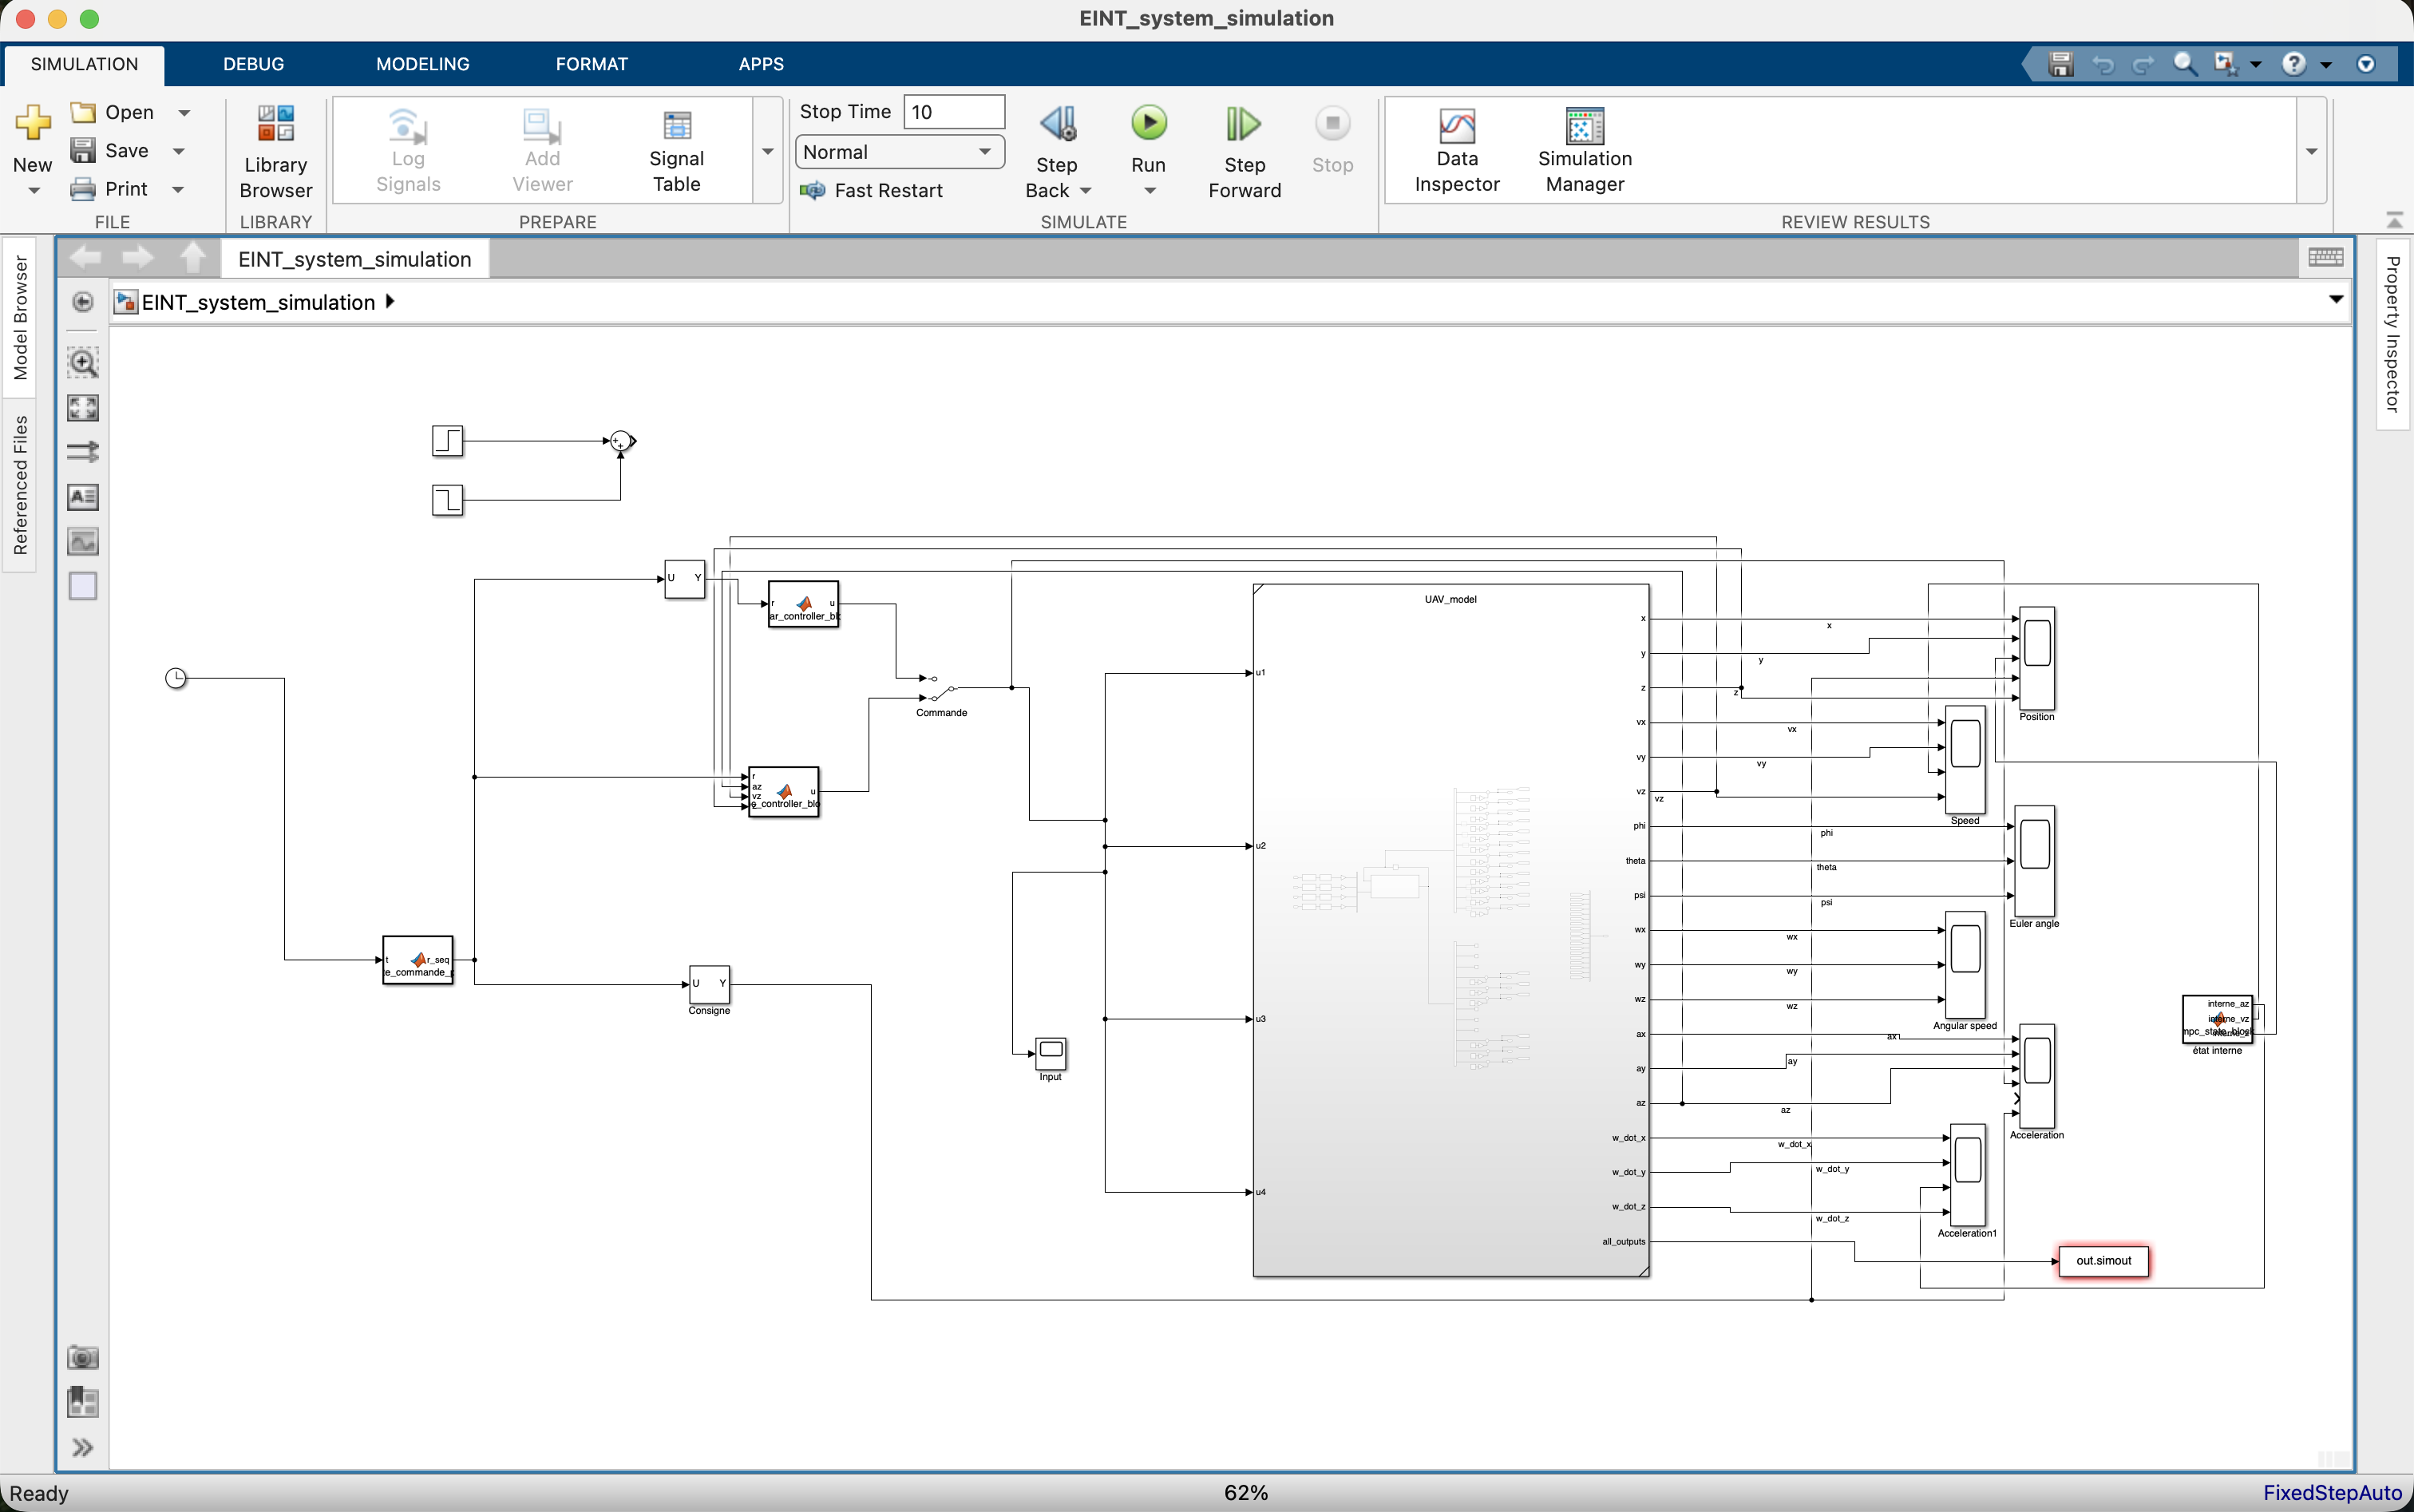
\includegraphics[width=\paperwidth]{screen_simulink.png}
        };
    \end{tikzpicture}%
}
\begin{frame}[plain,noframenumbering]
    \titlepage
\end{frame}
}

% ------------------------------------------------------------------------------
% Table of Contents Slide
% ------------------------------------------------------------------------------
{
\setbeamertemplate{headline}{}
\begin{frame}[noframenumbering]{Table of Contents}
    \small
    \tableofcontents[hideallsubsections]
\end{frame}
}

% ==============================================================================
% SECTIONS MODULAIRES
% ==============================================================================
% ==============================================================================
% SECTION 1: INTRODUCTION AND CONTEXT
% ==============================================================================
\section{Introduction}

\begin{frame}{Project Objectives}
    \begin{columns}[c]
        % --- Left Column: Text Area ---
        \begin{column}{0.52\textwidth}
            \textbf{Available Resources:}
            \begin{itemize}
                \item Dataset of vertical acceleration.
                \item MATLAB/Simulink drone simulator.
            \end{itemize}

            \vspace{0.4em}
            \textbf{Objectives:}
            \begin{itemize}
                \item Validate the dataset.
                \item Identify the model.
                \item Develop a control law.
            \end{itemize}

        \end{column}

        % --- Right Column: 3 figures step_1, step_2, step_3 ---
        \begin{column}{0.45\textwidth}
            \centering
            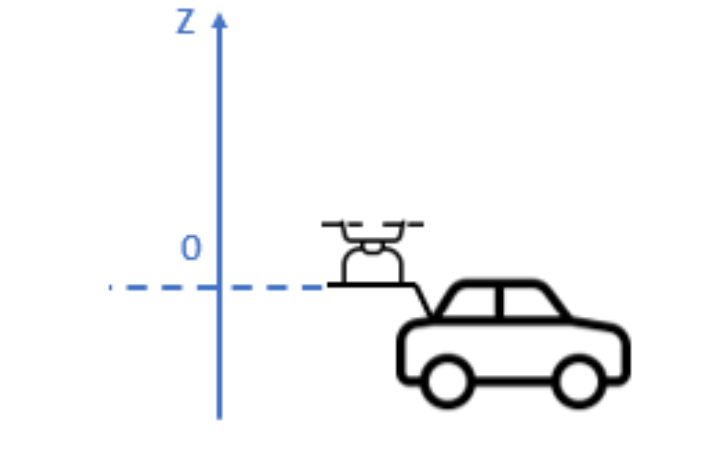
\includegraphics[width=\linewidth, height=2.1cm, keepaspectratio]{step_1.png}
            \vspace{0.3em}

            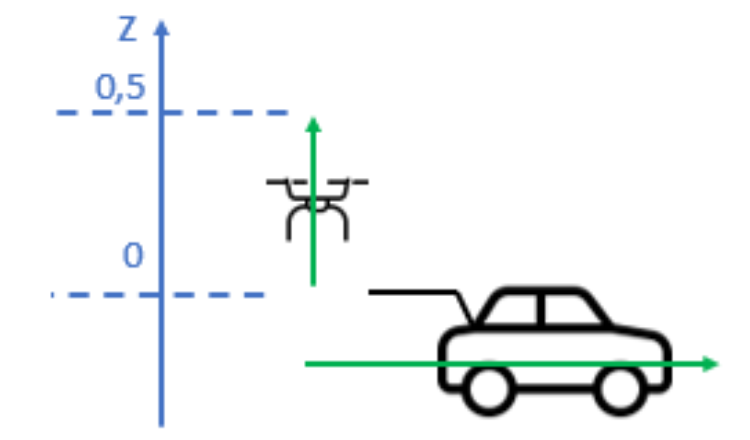
\includegraphics[width=\linewidth, height=2.1cm, keepaspectratio]{step_2.png}
            \vspace{0.3em}

            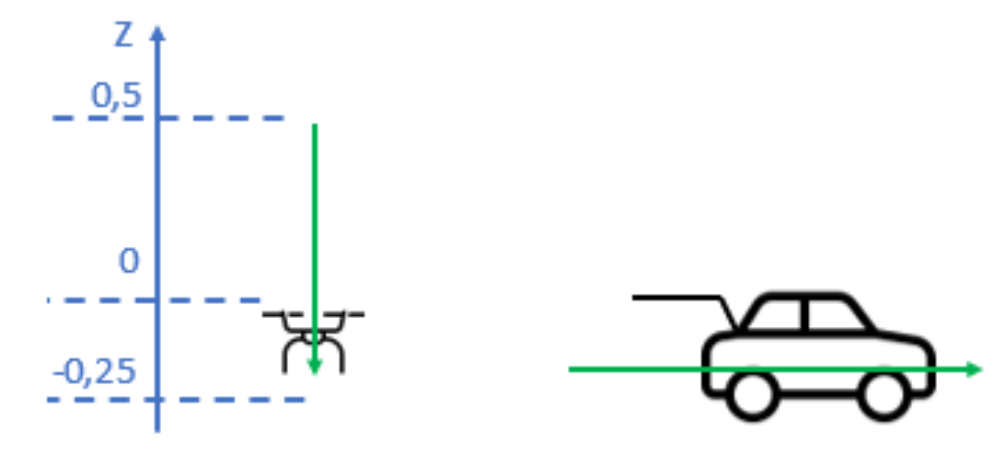
\includegraphics[width=\linewidth, height=2.1cm, keepaspectratio]{step_3.png}
        \end{column}
    \end{columns}
\end{frame}

% ==============================================================================
% SECTION 2: VALIDATION OF THE DATASET
% ==============================================================================
\section{Dataset Validation}

\begin{frame}{Dataset Validation}
    \begin{columns}[T]
        % --- Left Column: Filtering Criteria ---
        \begin{column}{0.54\textwidth}

            \begin{block}{Cleaning the data}
                \textbf{Remove lines that includes:}
                \begin{itemize}
                    \item Frozen sensor for 2+ seconds 
                    \item 5+ diverging values
                \end{itemize}
            \end{block}

            \begin{block}{Normalisation}
                \begin{itemize}
                    \item Directly in the training 
                \end{itemize}
            \end{block}

        \end{column}

        % --- Right Column: Visual Result / Impact ---
        \begin{column}{0.44\textwidth}
            
            \begin{block}{Static characteristic}
                \centering
                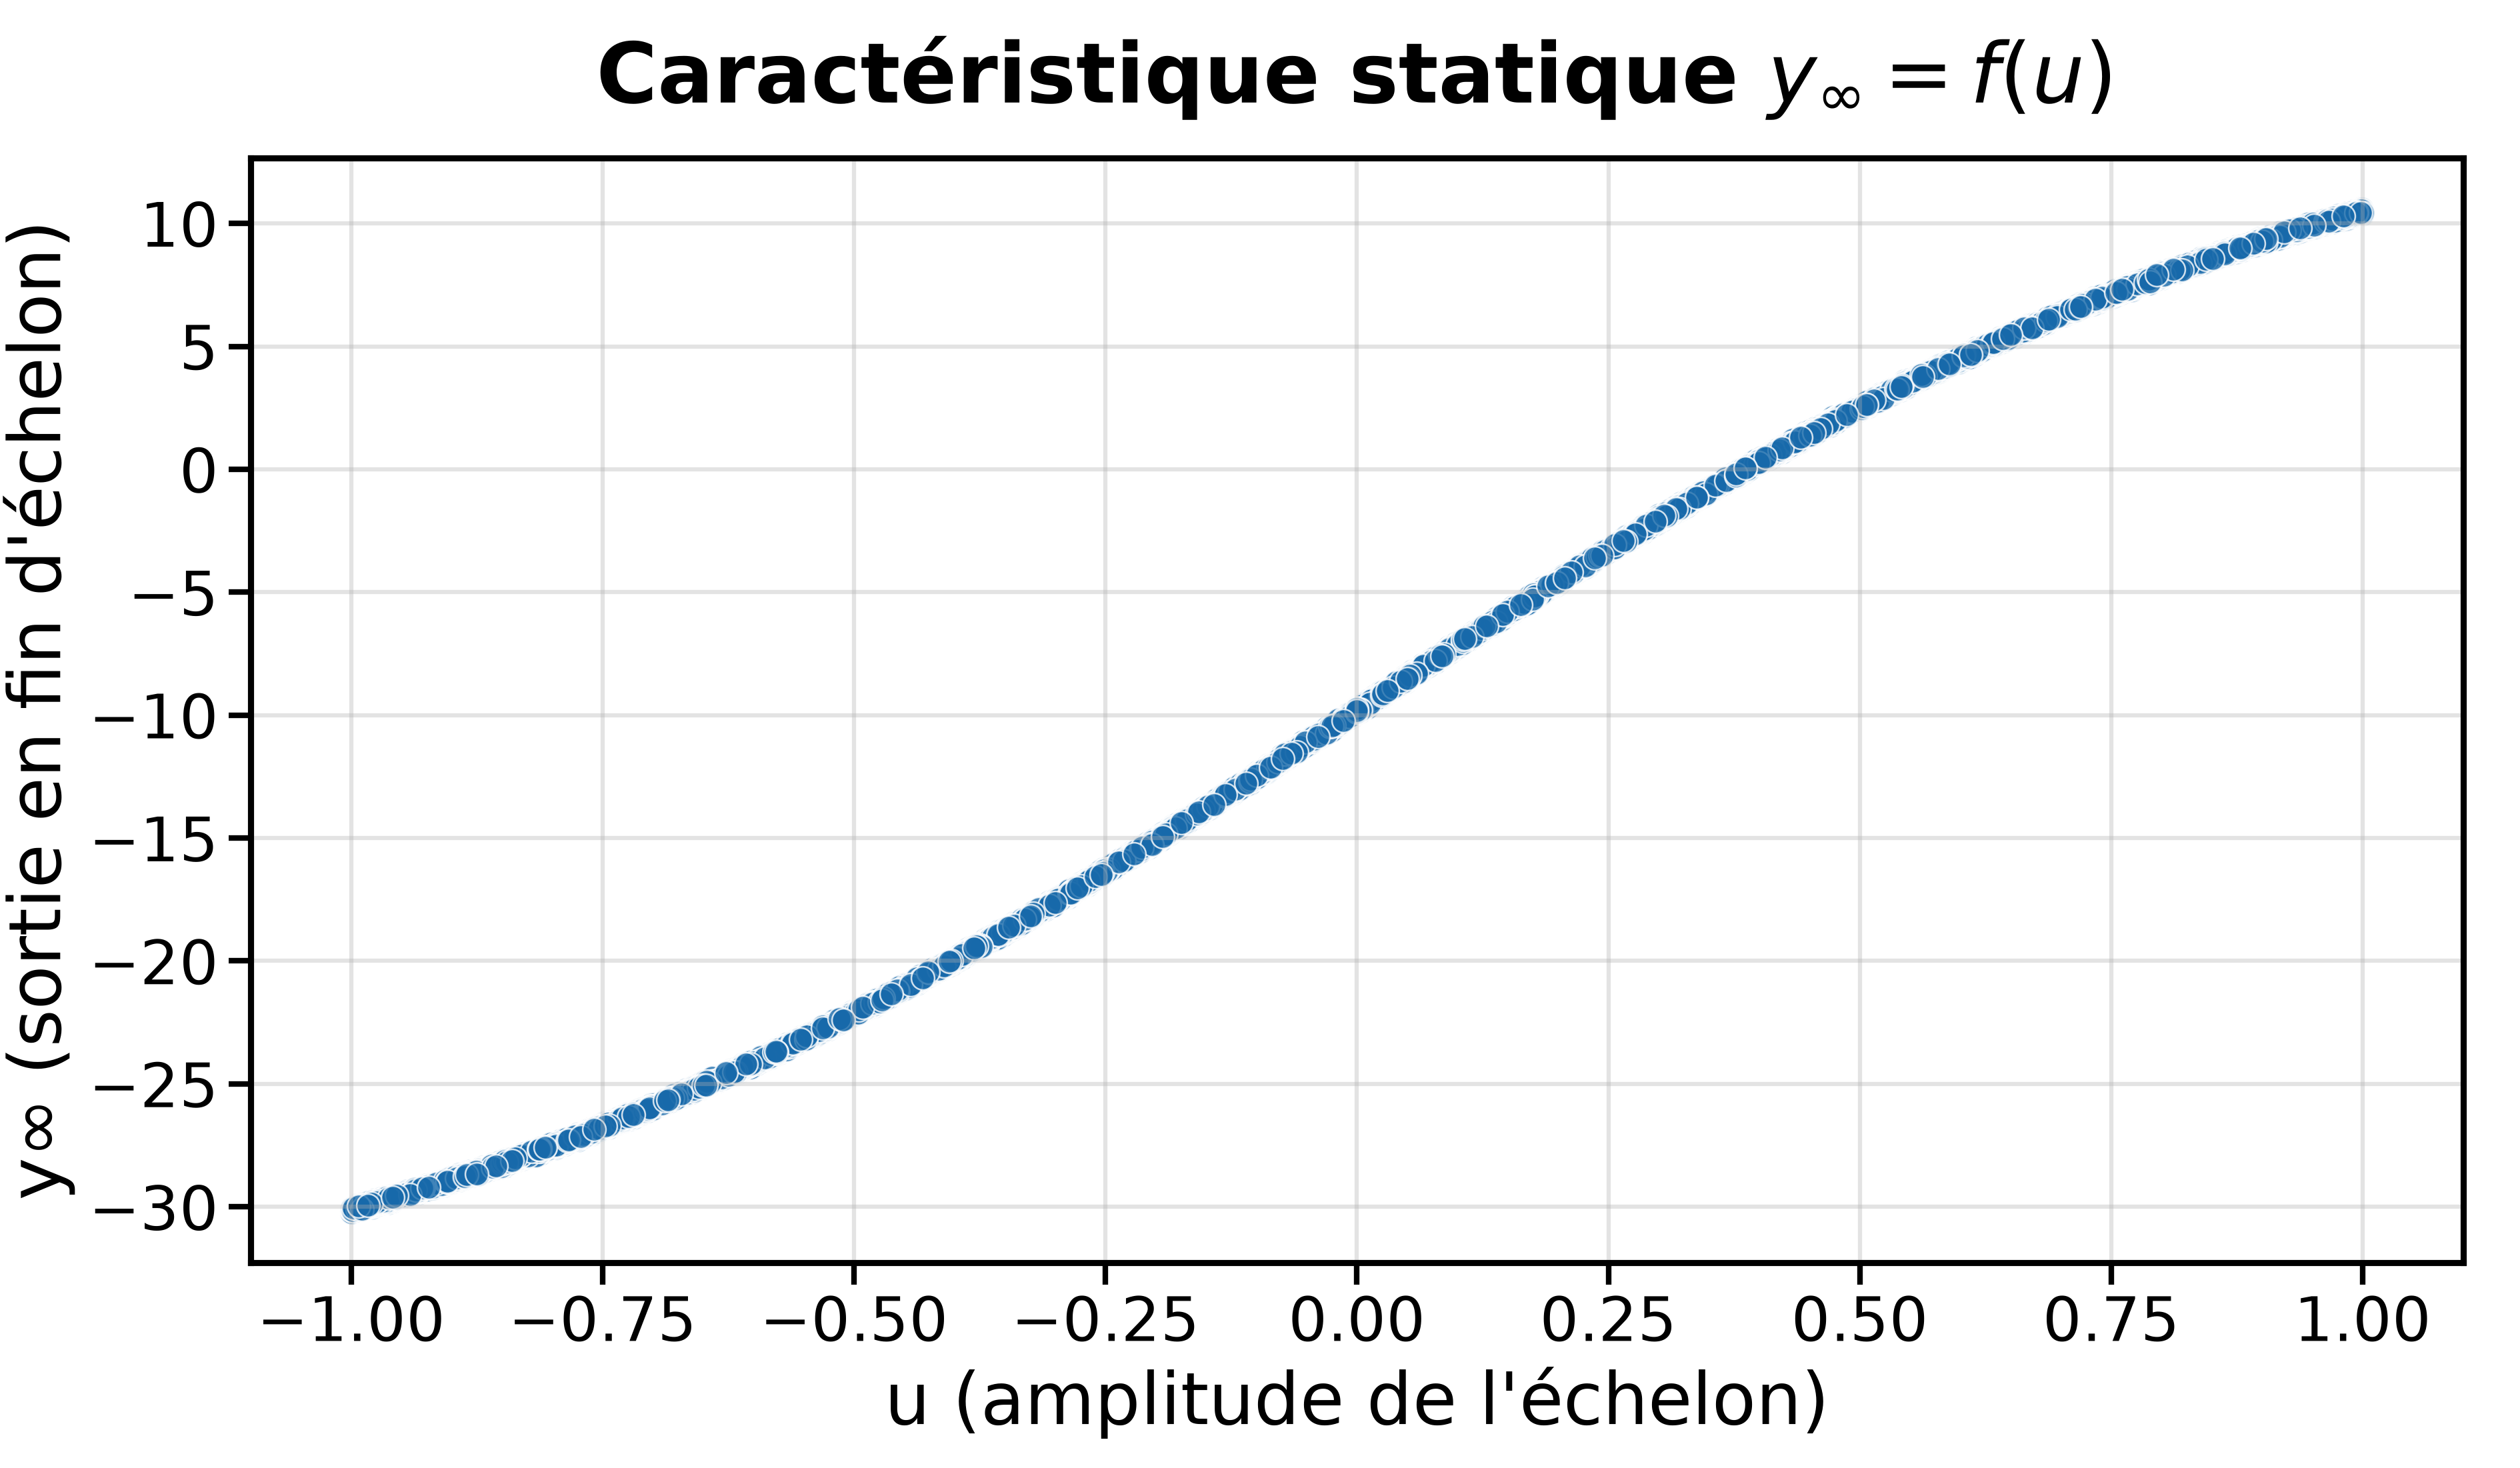
\includegraphics[
                    width=\linewidth,
                    height=5.0cm,
                    keepaspectratio
                ]{dataset_static_characteristic.png}
                % \vspace{0.1em}
                
                {\scriptsize $y_\infty = f(u)$ after eliminating corrupted runs.}
            \end{block}

        \end{column}
    \end{columns}
\end{frame}

\section{System Modeling}
% ==============================================================================
% SECTION 2: LINEAR MODELING & IDENTIFICATION
% ==============================================================================
\begin{frame}{System Modeling}
    \framesubtitle{Linear Model: Hammerstein Approach}
    \begin{columns}[T]
        \begin{column}{0.5\textwidth}
            \begin{block}{Static Characteristic $N(u)$}
                3rd-order polynomial identified on steady-state regimes:
                \begin{equation*}
                    v(t) = N(u) = a_3 u^3 + a_2 u^2 + a_1 u + a_0
                \end{equation*}
                \textbf{Tau identification}
            \end{block}
        \end{column}

        \begin{column}{0.5\textwidth}

                \centering
                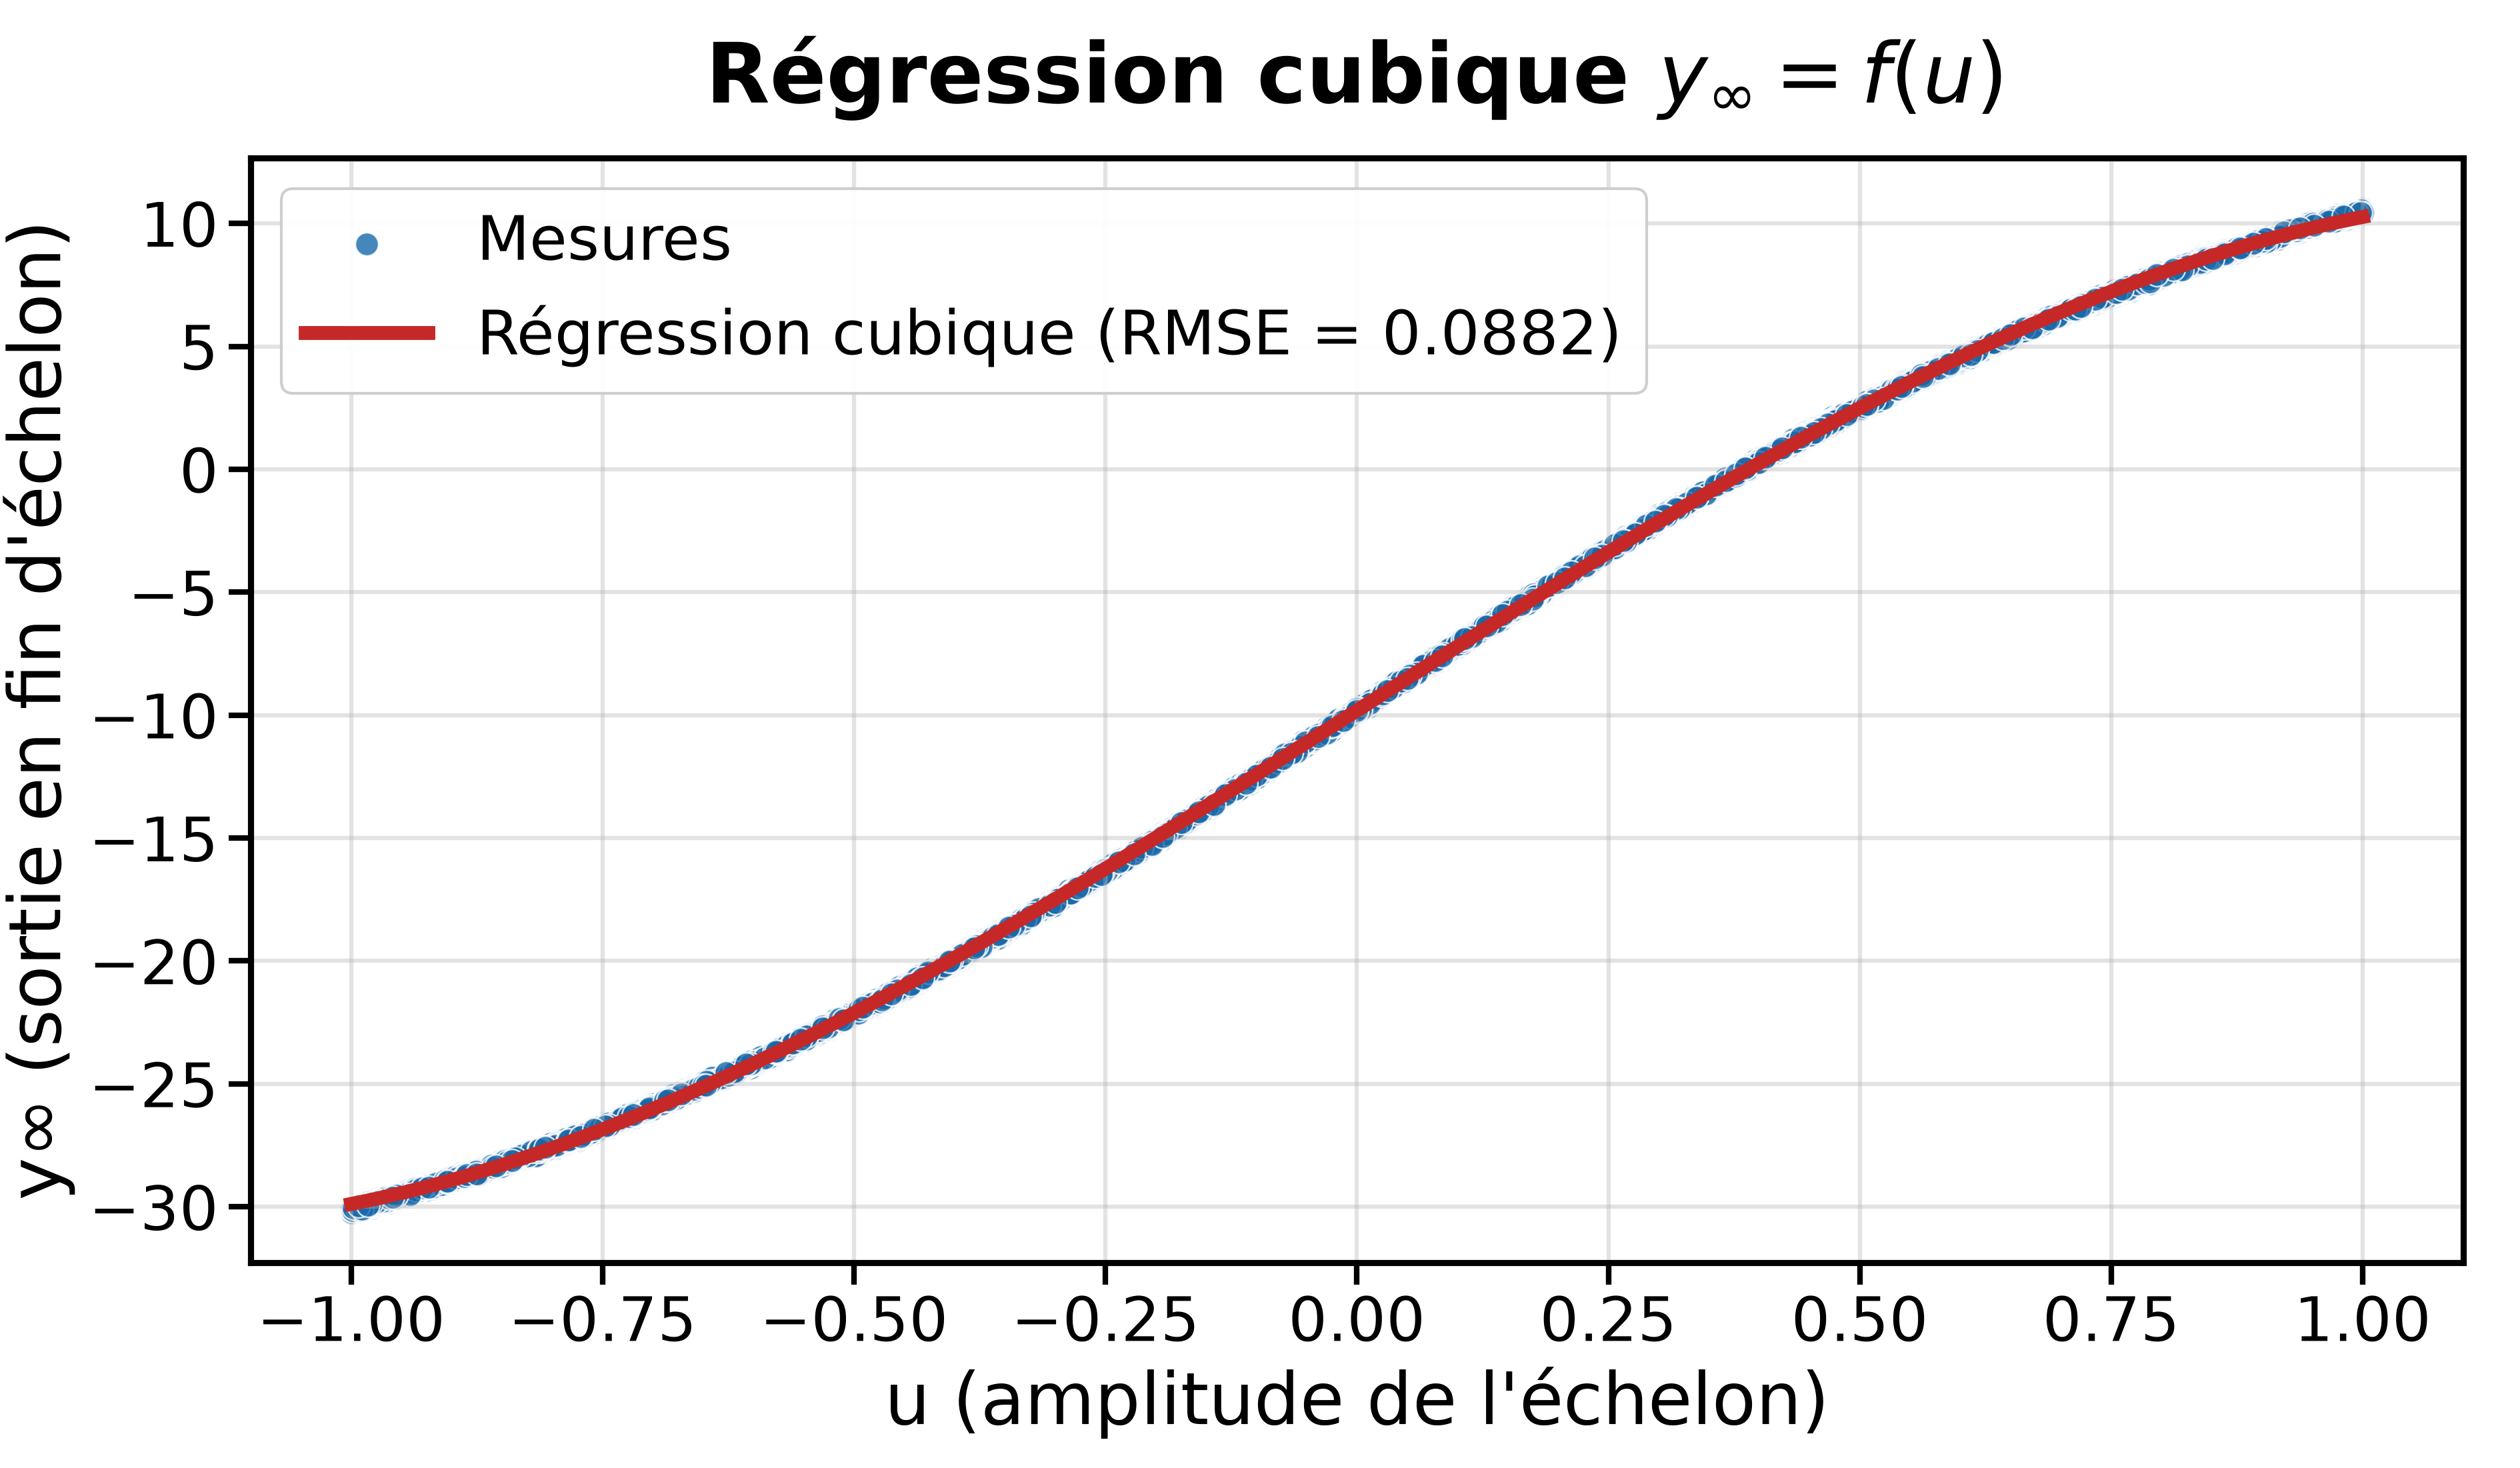
\includegraphics[
                    width=\linewidth,
                    height=2.6cm,
                    keepaspectratio
                ]{regression sur caracteristique statique.png}


                \centering
                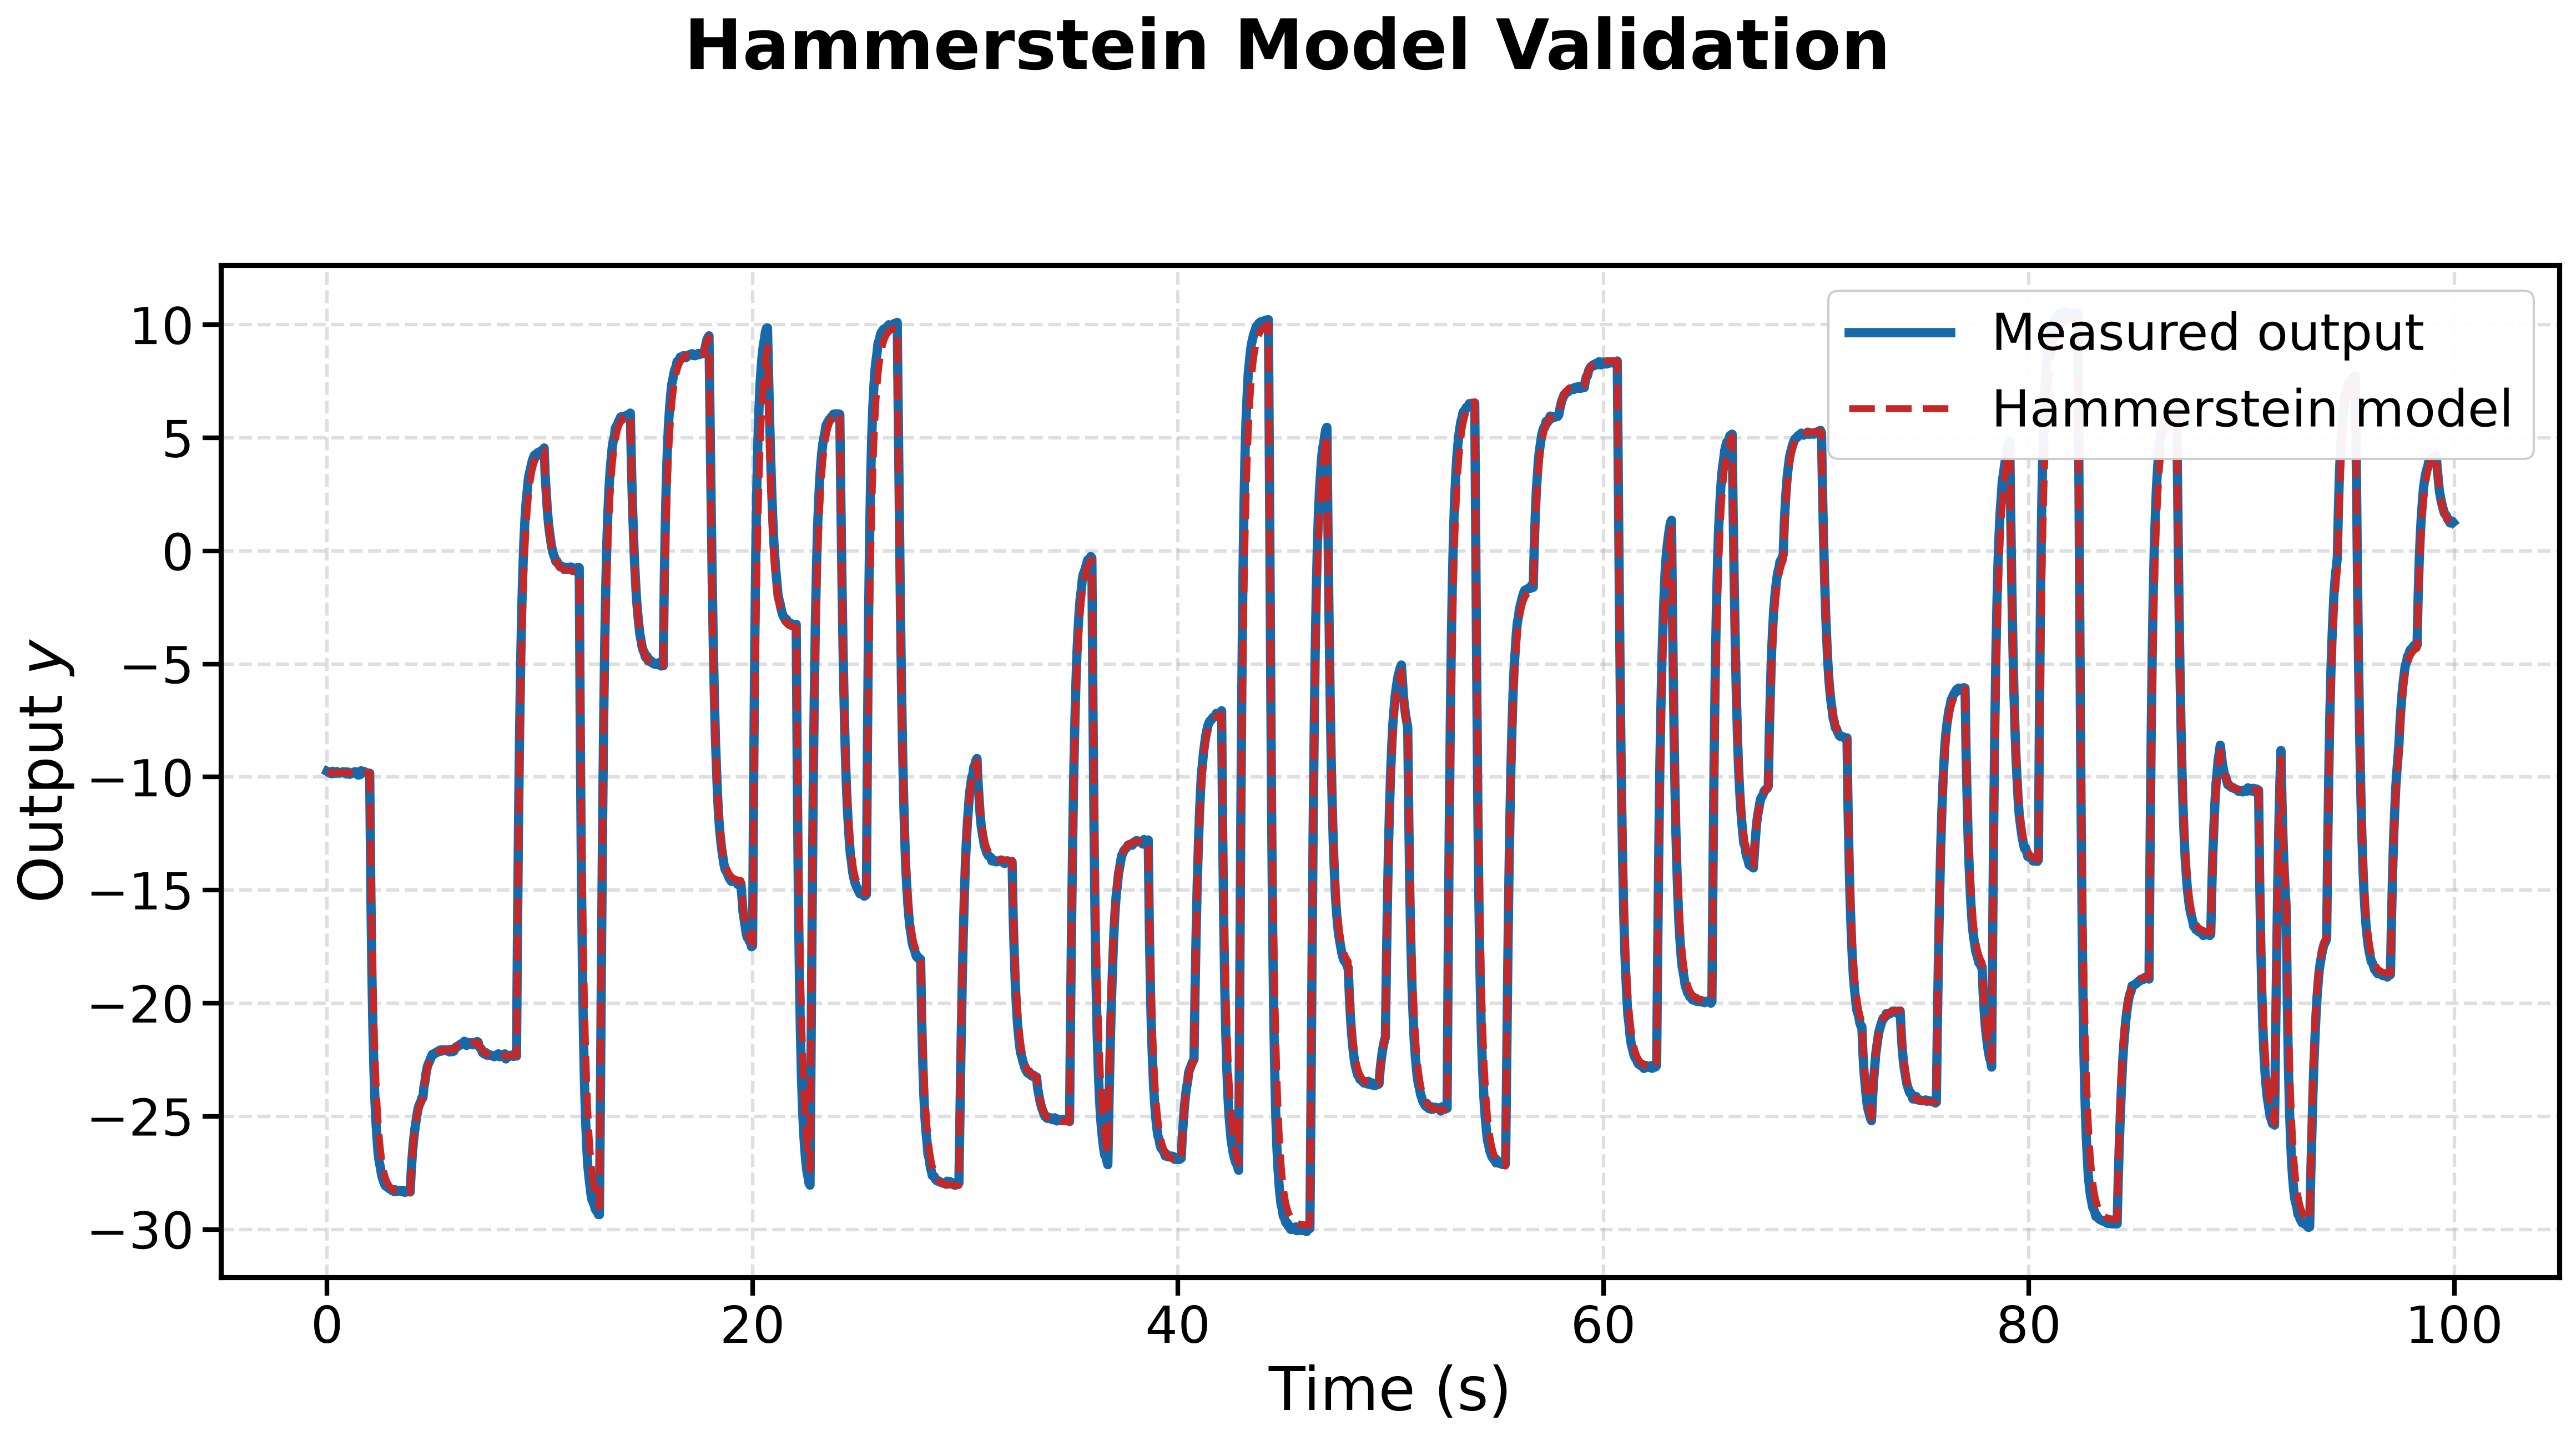
\includegraphics[
                    width=\linewidth,
                    height=5.0cm,
                    keepaspectratio
                ]{hammerstein_model_validation.png}
                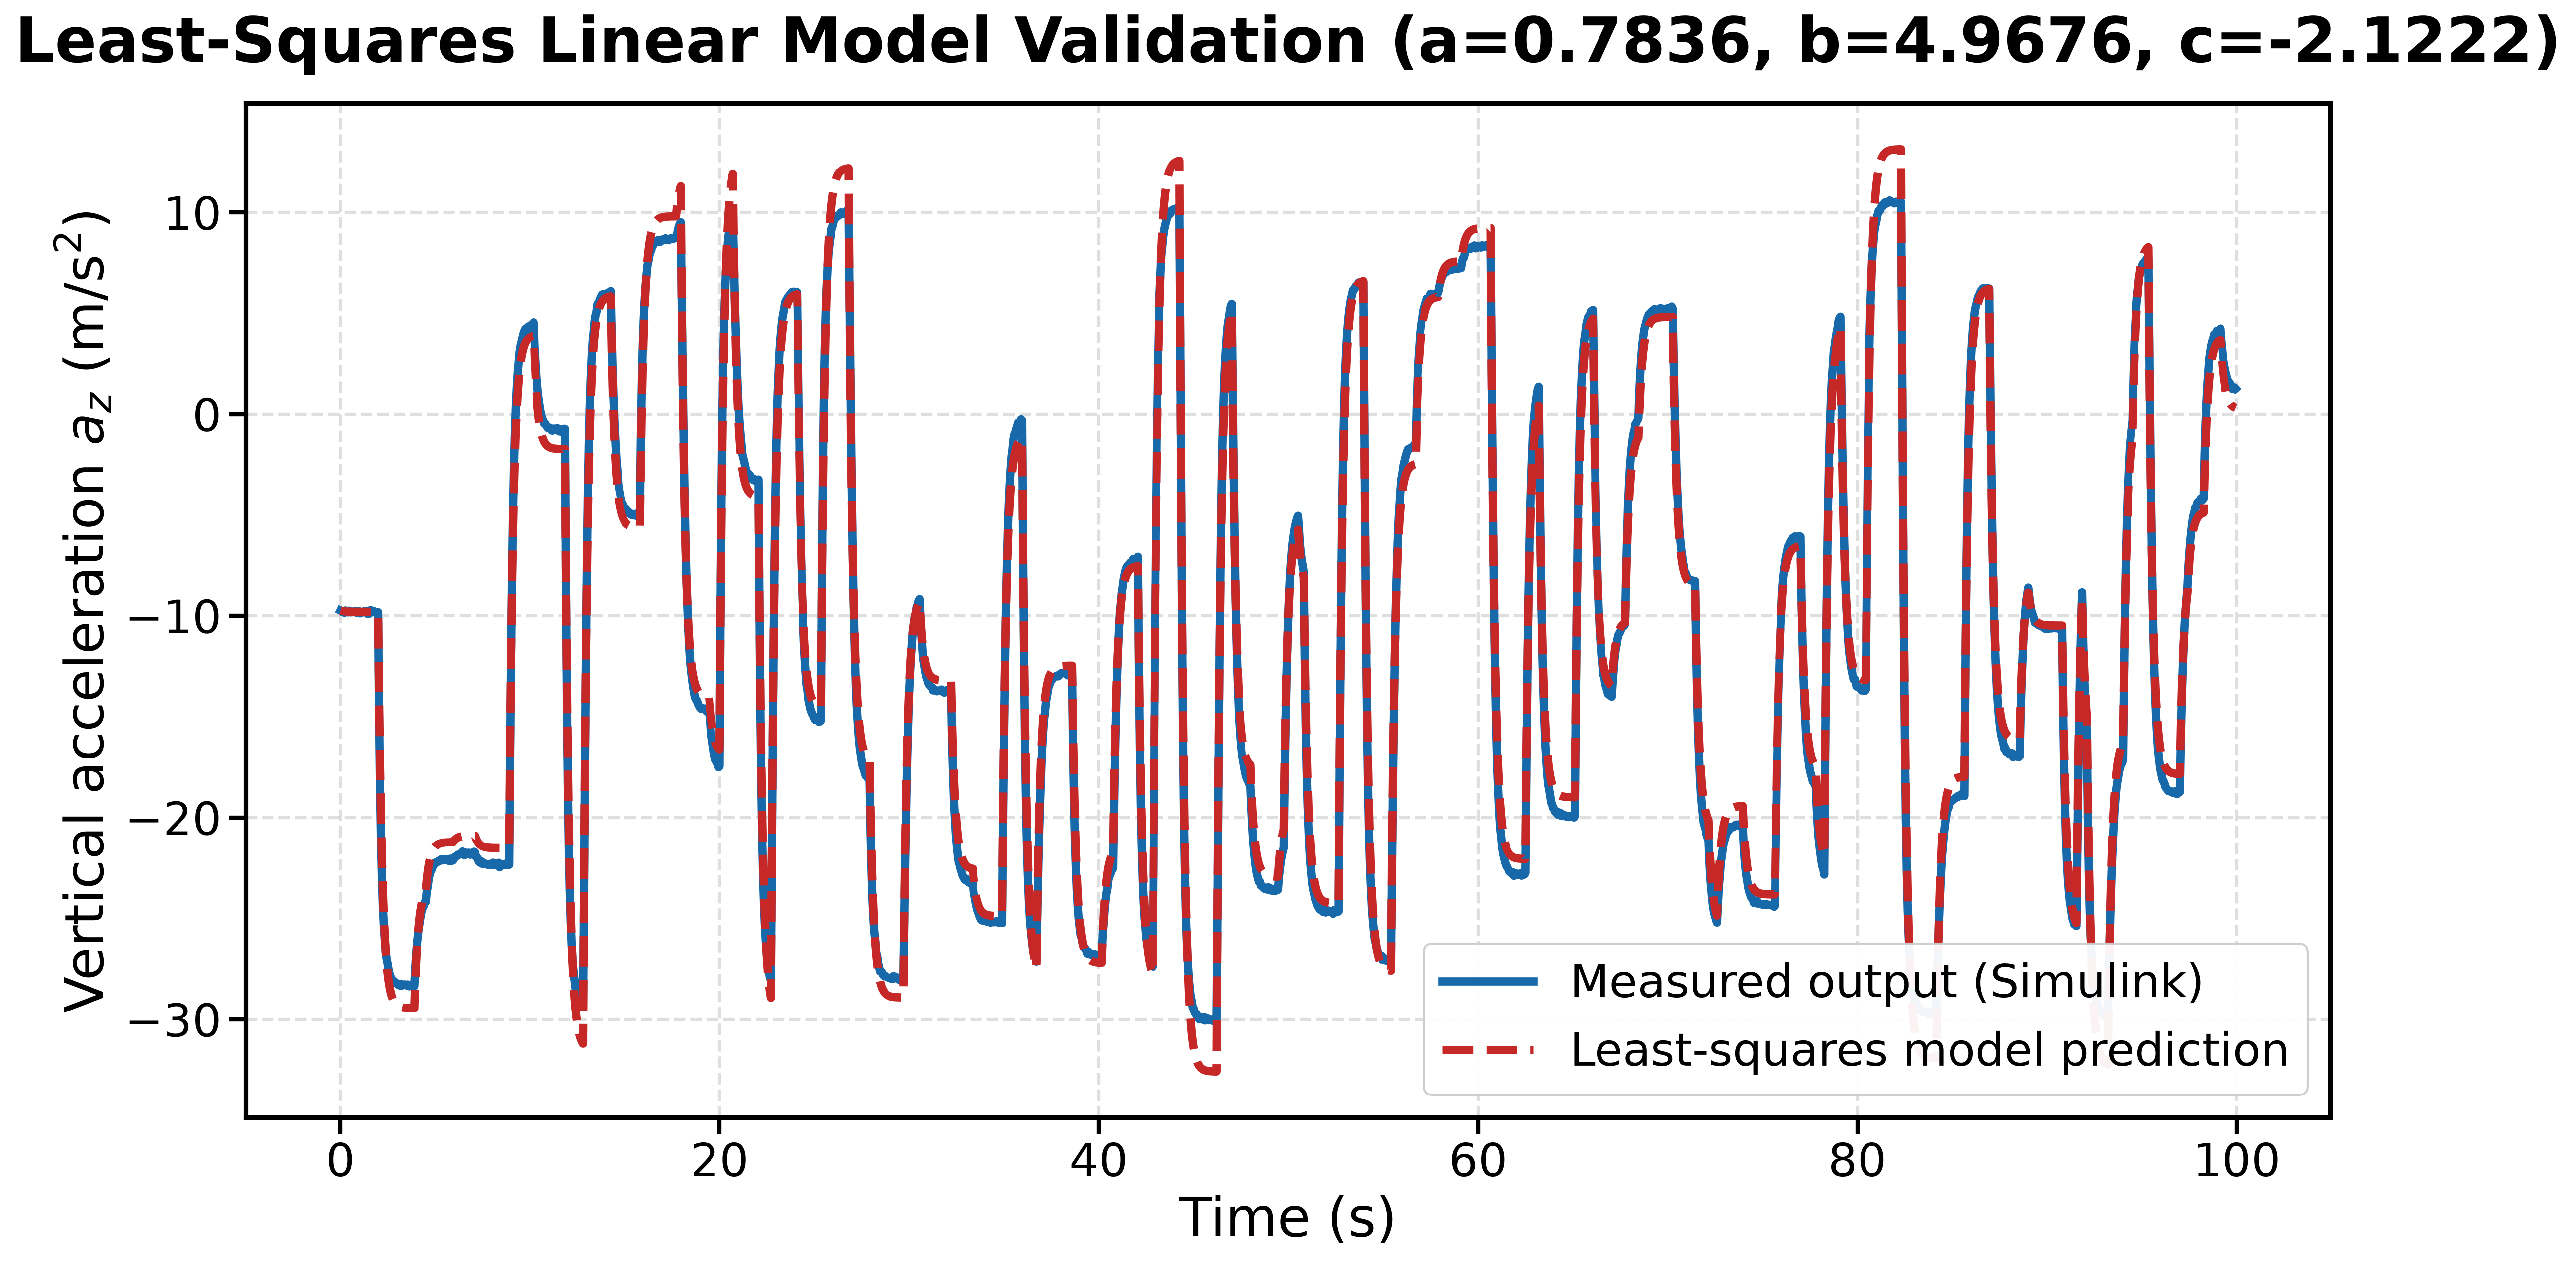
\includegraphics[
                width=\linewidth,
                height=2.75cm,
                keepaspectratio
            ]{least_squares_model_validation.png}
        \end{column}
    \end{columns}
\end{frame}

\begin{frame}{System Modeling}
    \framesubtitle{Linear Model: Least Square Method}
    \begin{columns}[T]
        \begin{column}{0.52\textwidth}

            \begin{block}{Model equations}
                \begin{align*}
                    y_k(t+1)
                        &= a\,y_k(t) + b\,u_k(t) + c \\
                        &= \boldsymbol{\varphi}_k^{\mathsf T}
                           \boldsymbol{\theta}.
                \end{align*}
                \[
                    \boldsymbol{\varphi}_k^{\mathsf T} =
                    \begin{bmatrix} y_k(t) & u_k(t) & 1 \end{bmatrix}
                    \qquad
                    \boldsymbol{\theta} =
                    \begin{bmatrix} a & b & c \end{bmatrix}^{\mathsf T}.
                \]

                The least-squares estimate is
                \begin{equation*}
                    \boldsymbol{\theta}^{\star}
                        =
                        \left(\boldsymbol{\Phi}^{\mathsf T}
                        \boldsymbol{\Phi}\right)^{-1}
                        \boldsymbol{\Phi}^{\mathsf T}\boldsymbol{Y}.
                \end{equation*}
            \end{block}
        \end{column}

        \begin{column}{0.48\textwidth}
            \centering

            \vspace{0.15cm}

            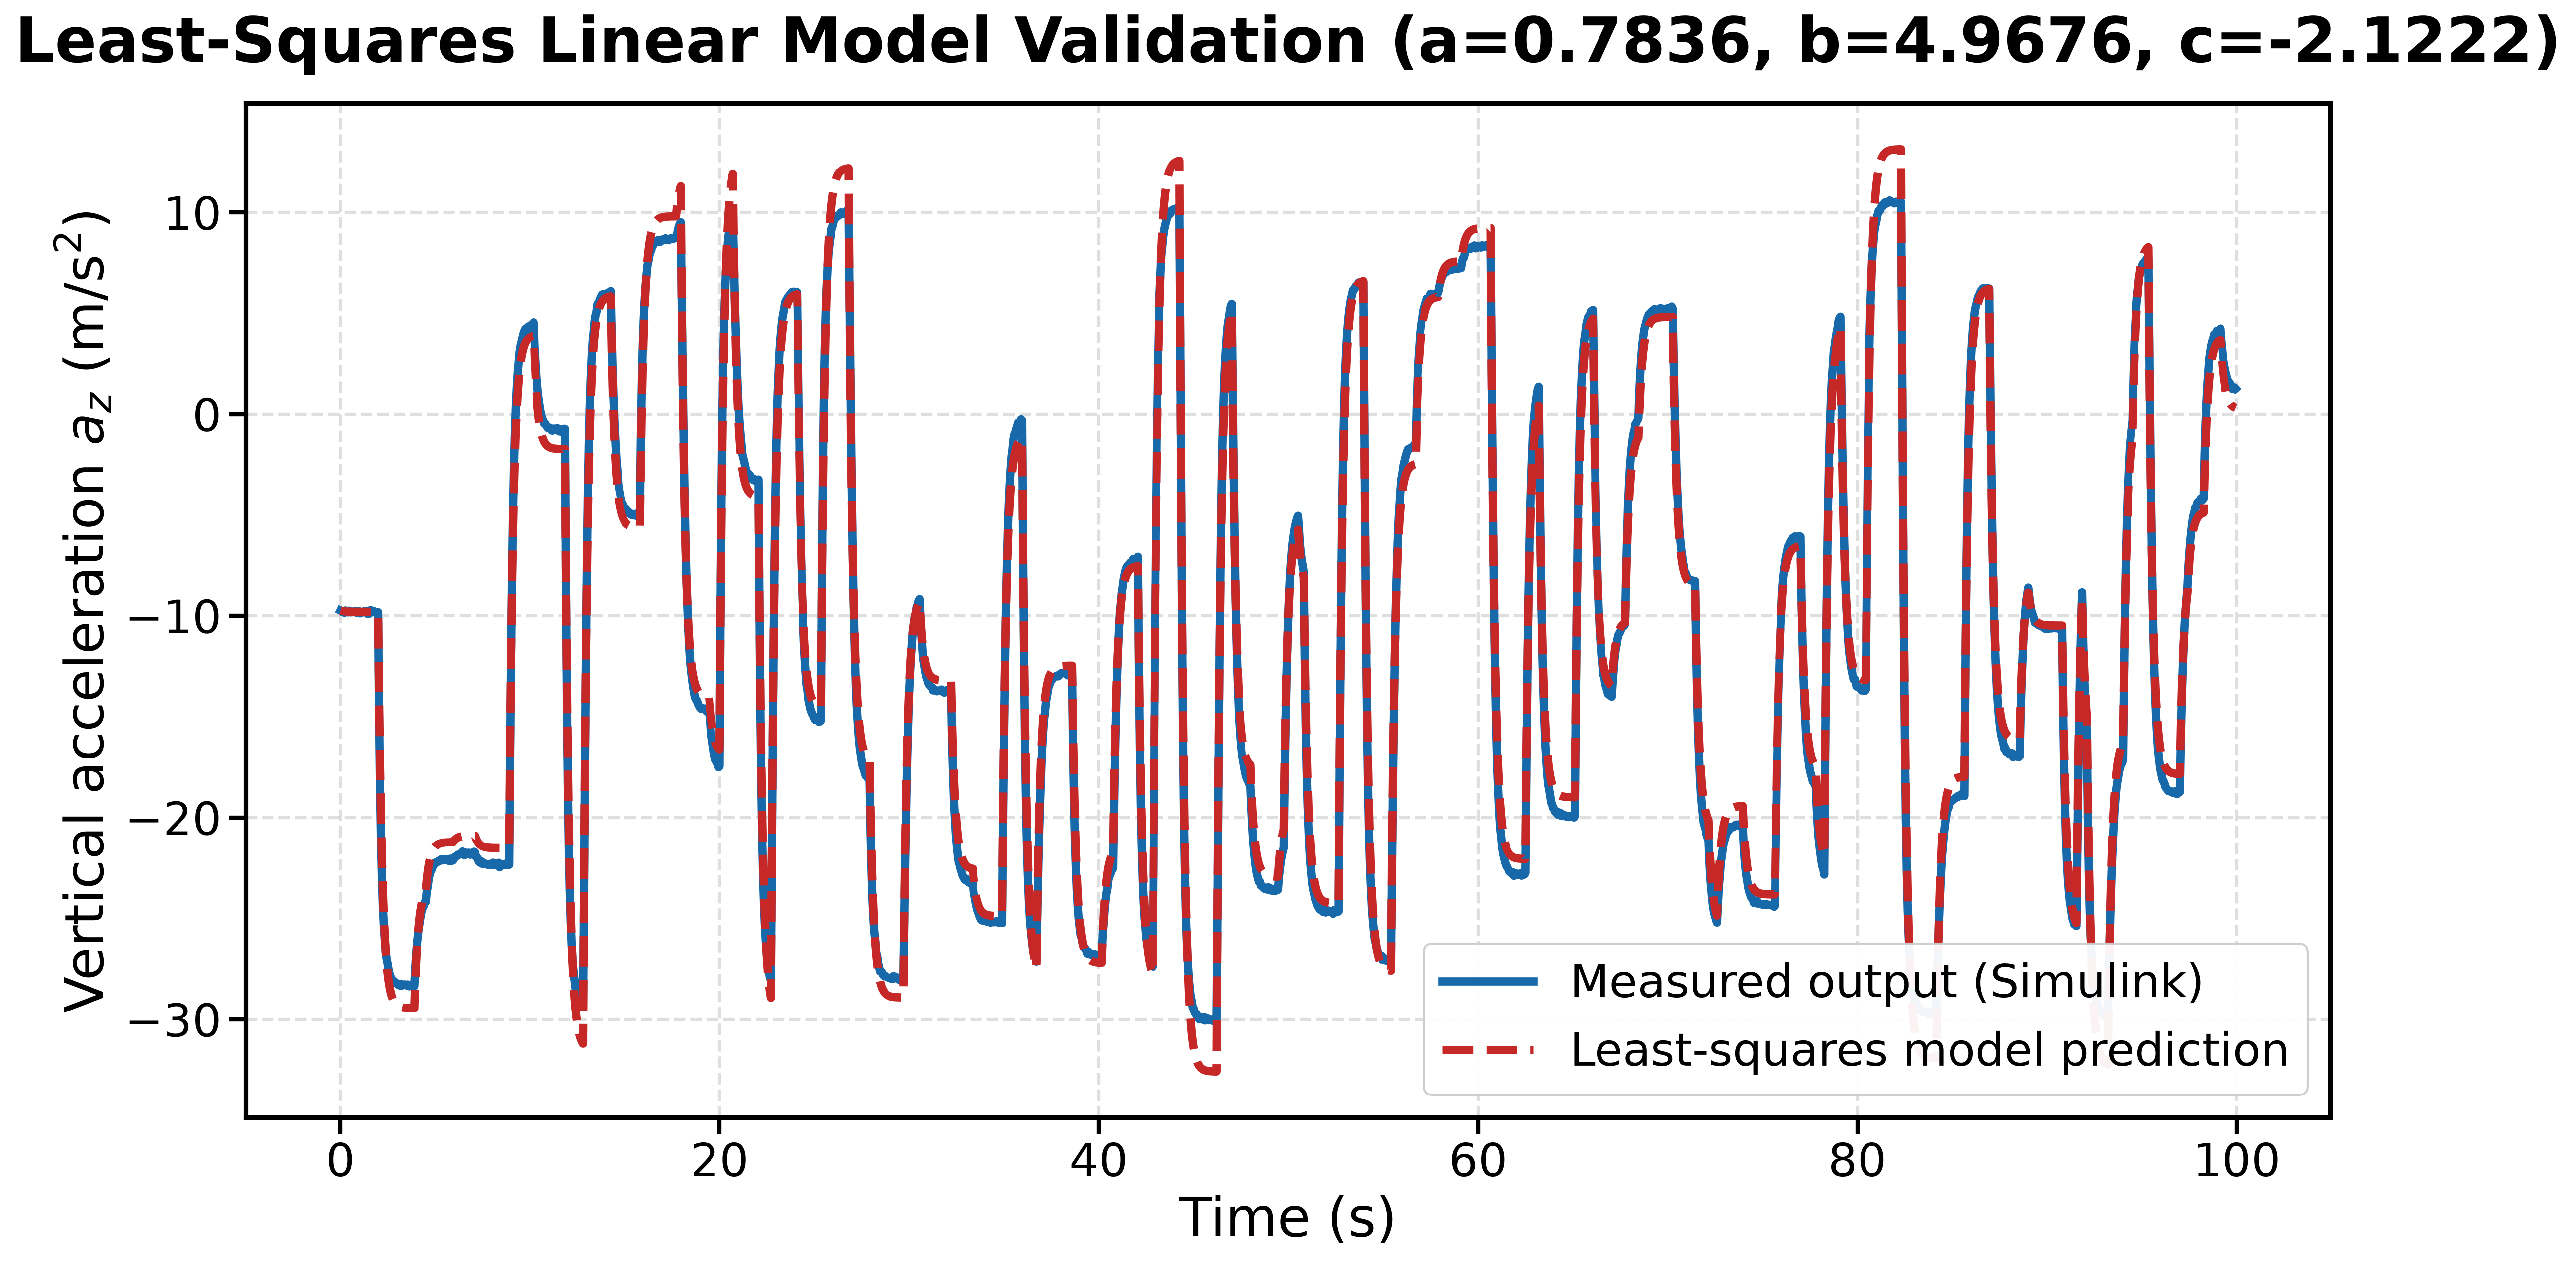
\includegraphics[
                width=\linewidth,
                height=2.75cm,
                keepaspectratio
            ]{least_squares_model_validation.png}
        \end{column}
    \end{columns}
\end{frame}

% ==============================================================================
% SECTION 4: FIRST RECURRENT NEURAL NETWORK
% ==============================================================================
\section{First RNN}

\begin{frame}{First RNN}
    \framesubtitle{Sequence-to-sequence architecture}
    
    \begin{columns}[T]
        \begin{column}{0.48\textwidth}
            \begin{block}{Parameters}
                \begin{itemize}
                    \item One scalar input $u_t$ and one scalar output $\hat{y}_t$
                    \item   \begin{block}{Forward equations}
                                \begin{equation*}
                                    h_t = \tanh(W_{ih}u_t + W_{hh}h_{t-1} + b)
                                \end{equation*}
                                \begin{equation*}
                                    \hat{y}_t = W_{hy}h_t + b_y
                                \end{equation*}
                            \end{block}
                    \item Hidden state dimension: $16$
                    \item Early-stoppiong to avoid overfitting
                \end{itemize}
            \end{block}
        \end{column}

        \begin{column}{0.48\textwidth}
            \centering
            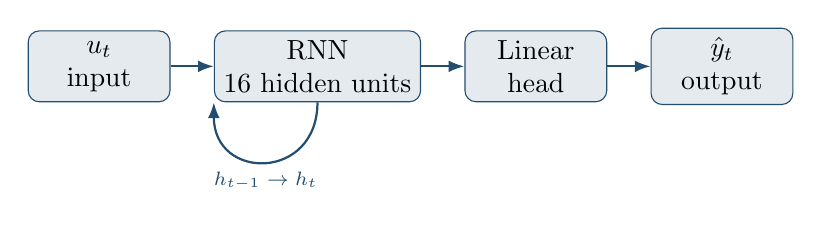
\begin{tikzpicture}[
                node distance=0.8cm and 0.55cm,
                box/.style={draw=CSSlate, fill=CSSlate!12, rounded corners,
                    minimum width=1.8cm, minimum height=0.9cm, align=center},
                arrow/.style={-{Latex[length=2mm]}, thick, CSSlate}
            ]
                \node[box] (input) {$u_t$\\input};
                \node[box, right=of input] (rnn) {RNN\\$16$ hidden units};
                \node[box, right=of rnn] (head) {Linear\\head};
                \node[box, right=of head] (output) {$\hat{y}_t$\\output};
                \draw[arrow] (input) -- (rnn);
                \draw[arrow] (rnn) -- (head);
                \draw[arrow] (head) -- (output);
                \draw[arrow] (rnn.south) .. controls +(0,-1.0) and +(0,-1.0)
                    .. node[below, font=\scriptsize] {$h_{t-1}\rightarrow h_t$} (rnn.south west);
            \end{tikzpicture}

        \end{column}

            \begin{block}{Least-squares criterion}
                \begin{equation*}
                    \hat{\boldsymbol{a}}
                    = \underset{\boldsymbol{a}}{\arg\min}
                    \sum_{i=1}^{N}
                    \left(y_{\infty,i} - \hat{y}_\infty(u_i)\right)^2
                \end{equation*}
            \end{block}

    \end{columns}
\end{frame}


\begin{frame}{First RNN}
    \framesubtitle{Results}
    \begin{columns}[T]

        \begin{column}{0.52\textwidth}
            \begin{block}{Numerical results}
                \begin{itemize}
                    \item Validation loss: $3.93\times 10^{-4}$
                    \item Test loss: $4.01\times 10^{-4}$
                    \item Training completed at epoch $100$
                    \item Only $321$ trainable parameters
                \end{itemize}
            \end{block}
        \end{column}

        \begin{column}{0.48\textwidth}
            \centering
            \vspace{0.15cm}
            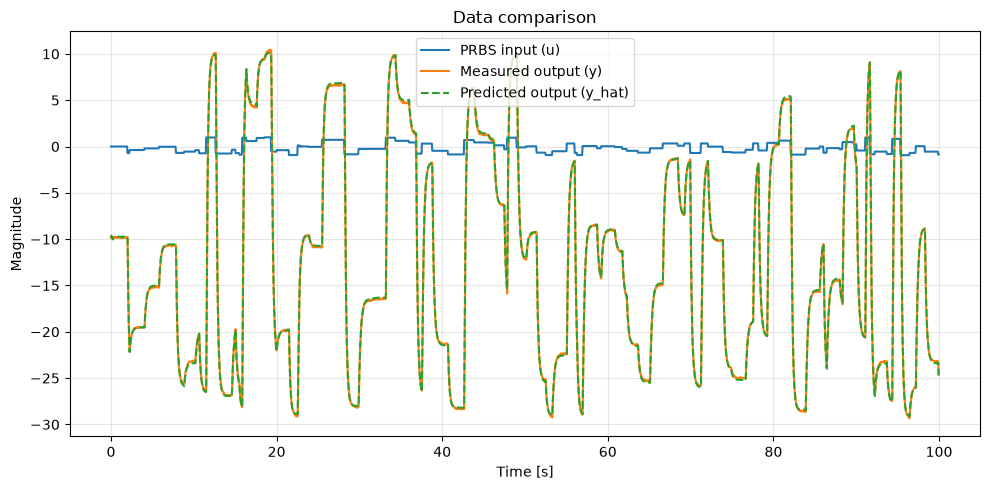
\includegraphics[
                width=0.92\textwidth,
                height=0.75\textheight,
                keepaspectratio
            ]{RNN1_results.png}
        \end{column}

    \end{columns}
\end{frame}
\section{Z-axis control}
% ==============================================================================
% MATLAB IMPLEMENTATION
% ==============================================================================

\begin{frame}{Z-axis control}
    \framesubtitle{Designing the command}

    \begin{columns}[T,onlytextwidth]
        \begin{column}{0.48\textwidth}
            \begin{block}{Principle}
                \begin{itemize}
                    \item Python Class Wrapping
                    \item Simulink Signal Generation
                    \item LQ control for the linear model
                    \item MPC control for the RNN
                \end{itemize}
            \end{block}

            \begin{exampleblock}{Results}
                Add here the main result or performance metric.
            \end{exampleblock}
        \end{column}

        \begin{column}{0.48\textwidth}
            \begin{block}{Figure}
                \centering
                % Replace the filename with the relevant figure.
                \fbox{%
                    \parbox[c][5.2cm][c]{0.9\linewidth}{%
                        \centering
                        \textit{Insert figure here}
                    }%
                }
            \end{block}
        \end{column}
    \end{columns}
\end{frame}

% ==============================================================================
% LQ CONTROL
% ==============================================================================

\begin{frame}{LQ control}
    \framesubtitle{Linear-quadratic control design}

    \begin{columns}[T,onlytextwidth]
        \begin{column}{0.48\textwidth}
            \begin{block}{Control principle}
                \centering
                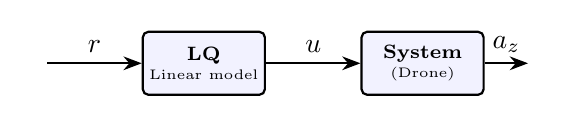
\begin{tikzpicture}[
                    auto,
                    >=Stealth,
                    thick,
                    node distance=1.2cm,
                    block/.style={
                        draw,
                        rectangle,
                        align=center,
                        minimum height=0.8cm,
                        minimum width=1.55cm,
                        inner sep=2pt,
                        fill=blue!5,
                        rounded corners=2pt,
                        font=\scriptsize
                    }
                ]
                    \node (reference) {};
                    \node[block, right=of reference] (lqr) {\textbf{LQ}\\[-1pt]\tiny Linear model};
                    \node[block, right=of lqr] (system) {\textbf{System}\\[-1pt]\tiny (Drone)};
                    \node[right=0.55cm of system] (output) {};

                    \draw[->] (reference) -- node {$r$} (lqr);
                    \draw[->] (lqr) -- node {$u$} (system);
                    \draw[->] (system) -- node {$a_z$} (output);
                \end{tikzpicture}
            \end{block}

            \begin{exampleblock}{Performance}
                \begin{itemize}
                    \item Global trajectory following
                    \item Wrong amplitude + phase shift
                    \item Missing prediction
                \end{itemize}
            \end{exampleblock}
        \end{column}

        \begin{column}{0.48\textwidth}
            \centering
            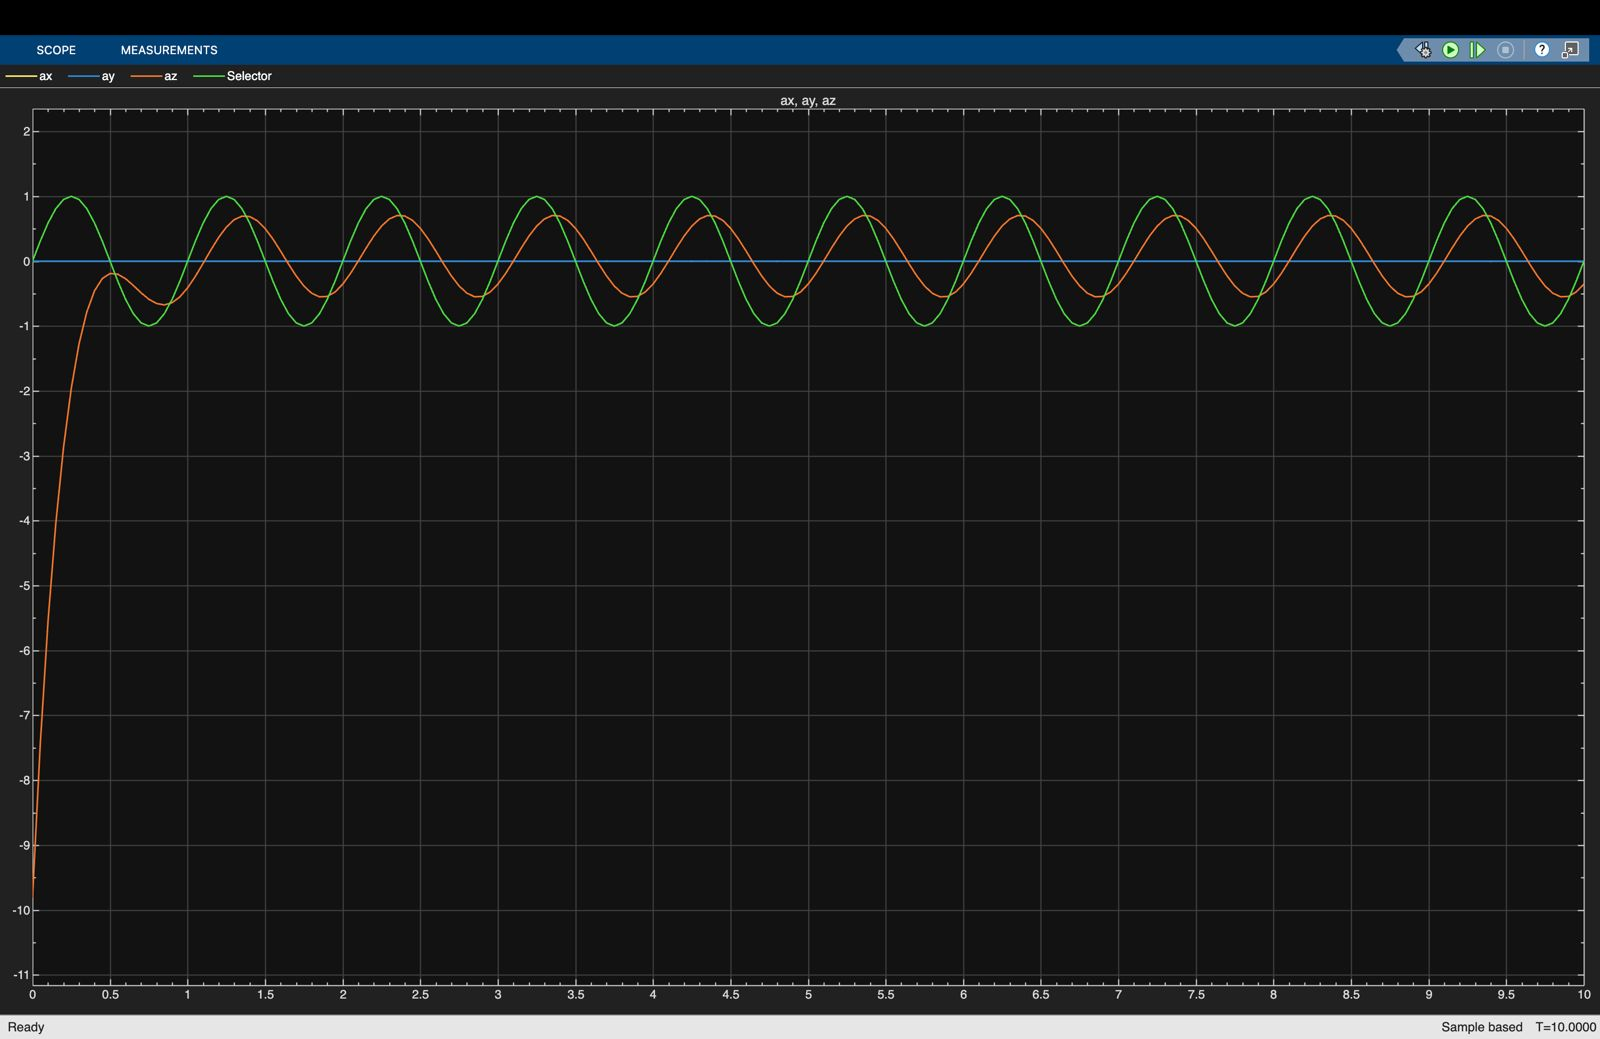
\includegraphics[
                width=\linewidth,
                height=5.5cm,
                keepaspectratio
            ]{lqr_linear_sinewave.jpeg}
        \end{column}
    \end{columns}
\end{frame}

% ==============================================================================
% MPC CONTROL
% ==============================================================================

\begin{frame}{MPC control}
    \framesubtitle{Model predictive control design}

    \begin{columns}[T,onlytextwidth]
        \begin{column}{0.48\textwidth}
            \begin{block}{Control principle}
                Replace this text with the main elements of the MPC controller:
                \begin{itemize}
                    \item Describe the prediction model.
                    \item Explain the prediction and control horizons.
                    \item Present the cost function and constraints.
                \end{itemize}
            \end{block}

            \begin{exampleblock}{Performance}
                Add here the main performance result or metric.
            \end{exampleblock}
        \end{column}

        \begin{column}{0.48\textwidth}
            \centering
            % Replace the filename with the relevant MPC figure.
            \fbox{%
                \parbox[c][5.5cm][c]{0.9\linewidth}{%
                    \centering
                    \textit{Insert MPC control figure here}
                }%
            }
        \end{column}
    \end{columns}
\end{frame}

% ==============================================================================
% MPC WITH EKF
% ==============================================================================

\begin{frame}{MPC with EKF}
    \framesubtitle{State estimation and predictive control}

    \begin{columns}[T,onlytextwidth]
        \begin{column}{0.45\textwidth}
            \begin{block}{Control principle}
                \centering
                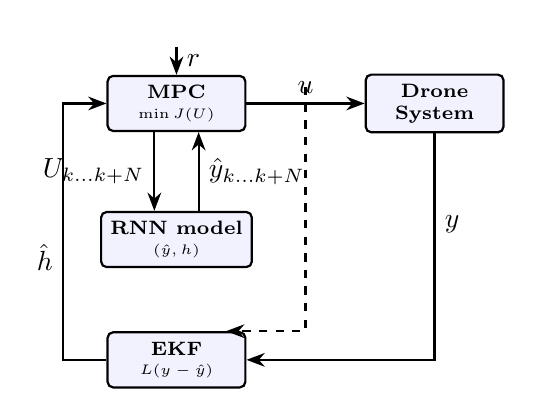
\begin{tikzpicture}[
                auto,
                >=Stealth,
                thick,
                node distance=1.4cm and 1.8cm,
                block/.style={
                    draw,
                    rectangle,
                    minimum height=0.7cm,
                    minimum width=1.75cm,
                    align=center,
                    fill=blue!5,
                    rounded corners=2pt,
                    font=\scriptsize
                }
            ]
                \node (ref) {};
                \node[block, below=0.35cm of ref] (mpc)
                    {\textbf{MPC}\\[-1pt]\tiny $\min J(U)$};
                \node[block, right=1.5cm of mpc] (system)
                    {\textbf{Drone} \\ \textbf{System}};
                \node[block, below=1.0cm of mpc] (rnn)
                    {\textbf{RNN model}\\[-1pt]\tiny $(\hat{y},h)$};
                \node[block, below=0.8cm of rnn] (ekf)
                    {\textbf{EKF}\\[-1pt]\tiny $L(y-\hat{y})$};

                \draw[->] (ref) -- node {$r$} (mpc);
                \draw[->] (mpc) -- node[name=u] {$u$} (system);
                \draw[->] (system.south) |- node[pos=0.2, right]
                    {$y$} (ekf.east);
                \draw[->, dashed] (u.center) |- (ekf.30);

                \draw[->] (ekf.west) -- ++(-0.55,0) |- node[pos=0.2, left]
                    {$\hat{h}$} (mpc.west);
                \draw[->] ([xshift=-8pt]mpc.south) --
                    node[left] {$U_{k \dots k+N}$} ([xshift=-8pt]rnn.north);
                \draw[->] ([xshift=8pt]rnn.north) --
                    node[right] {$\hat{y}_{k \dots k+N}$} ([xshift=8pt]mpc.south);
                \end{tikzpicture}
            \end{block}

            % \begin{exampleblock}{Performance}
            %     \begin{itemize}
            %         \item EKF-based state estimation improves feedback.
            %         \item The closed-loop response follows the sinusoidal
            %         reference more closely.
            %         \item The initial transient is reduced compared with the
            %         open-loop response.
            %     \end{itemize}
            % \end{exampleblock}
        \end{column}

        \begin{column}{0.55\textwidth}
            \centering
            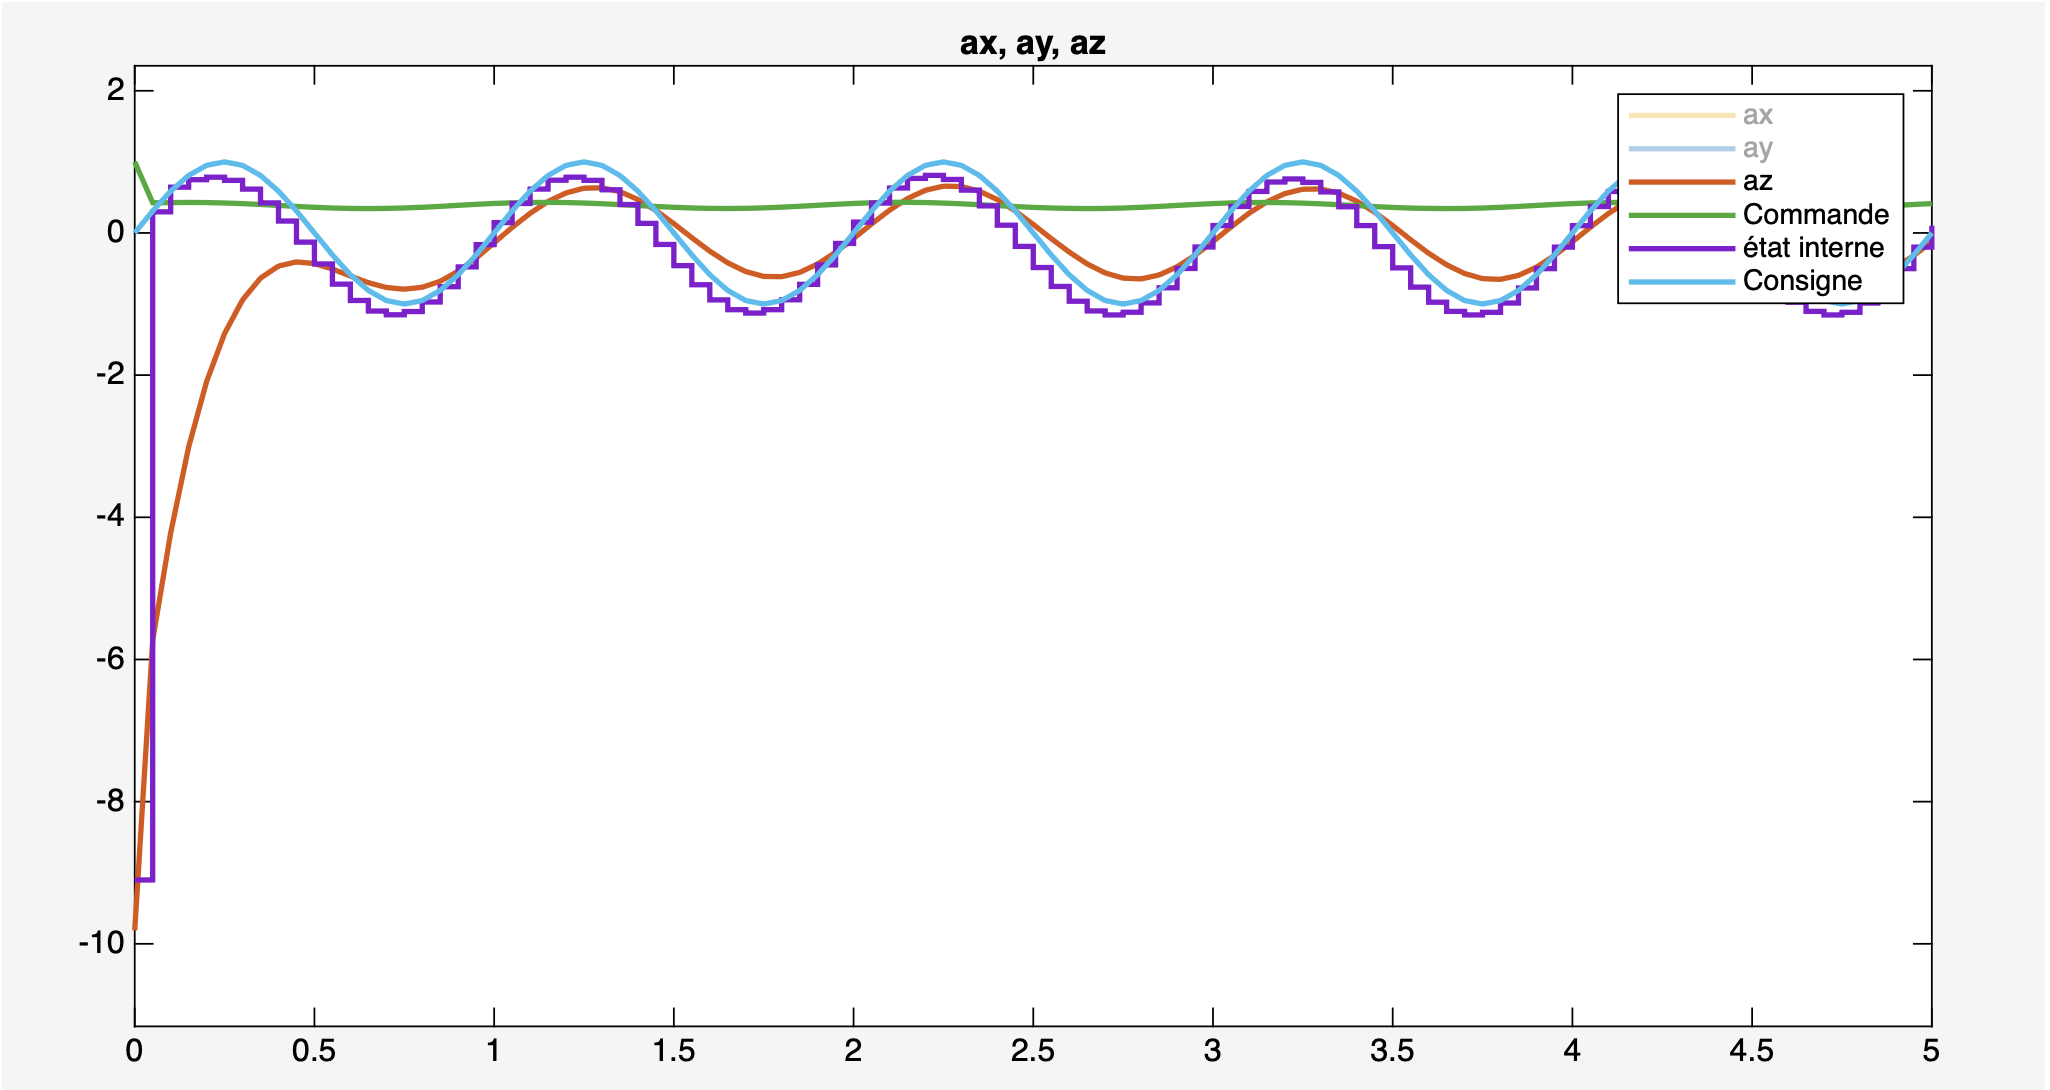
\includegraphics[
                width=\linewidth,
                height=0.38\textheight,
                keepaspectratio
            ]{sinus mpc boucle ouverte.png}

            \vspace{0.12cm}

            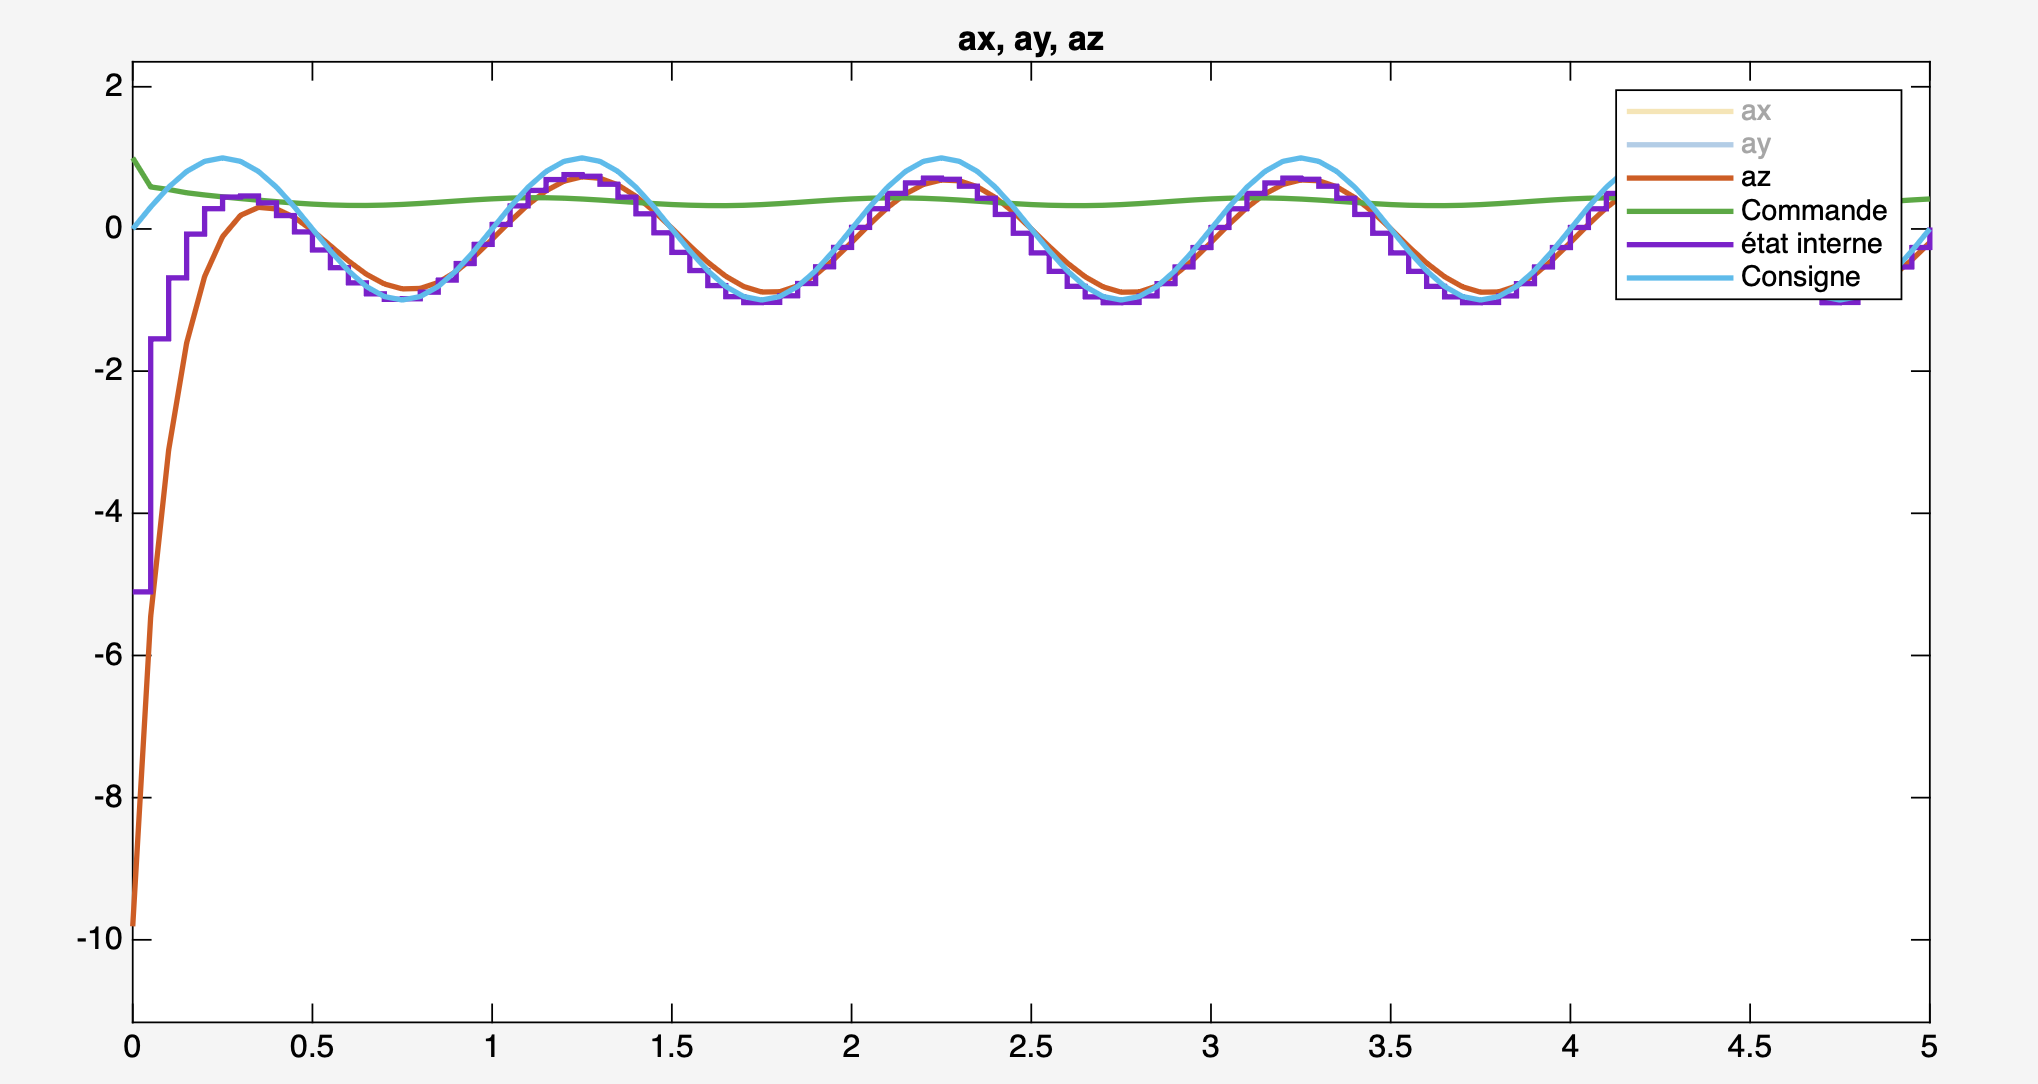
\includegraphics[
                width=\linewidth,
                height=0.38\textheight,
                keepaspectratio
            ]{sinus ekf mpc.png}
        \end{column}
    \end{columns}
\end{frame}

% ==============================================================================
% REQUESTED COMMAND WITH MPC AND EKF
% ==============================================================================

\begin{frame}{Requested command}
    \framesubtitle{MPC control with EKF feedback}

    \begin{columns}[T,onlytextwidth]
        \begin{column}{0.38\textwidth}
            \centering
            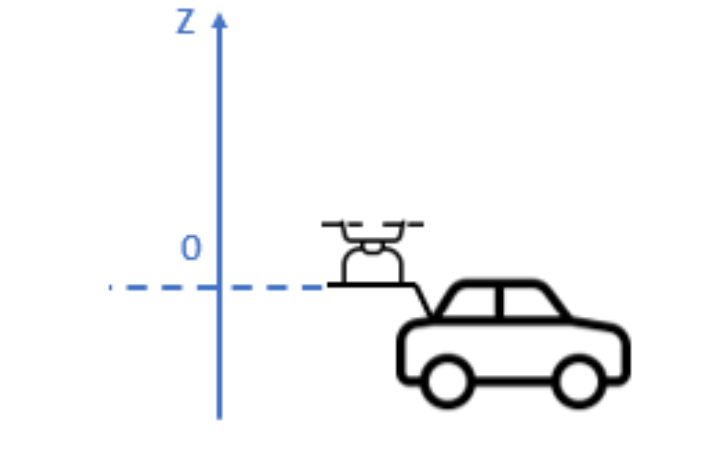
\includegraphics[
                width=\linewidth,
                height=1.65cm,
                keepaspectratio
            ]{step_1.png}

            \vspace{0.12cm}

            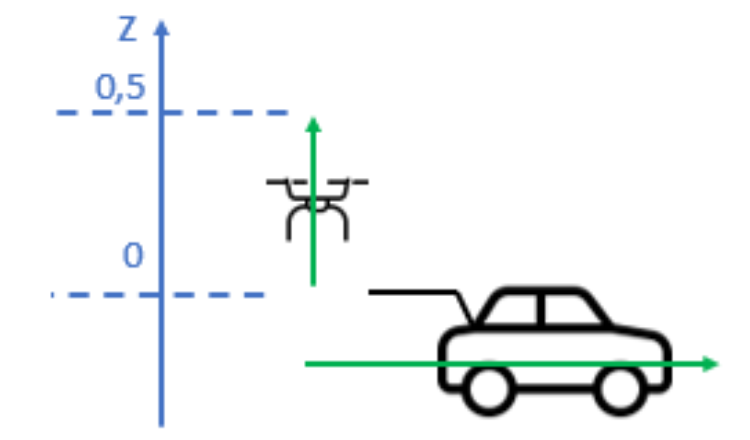
\includegraphics[
                width=\linewidth,
                height=1.65cm,
                keepaspectratio
            ]{step_2.png}

            \vspace{0.12cm}

            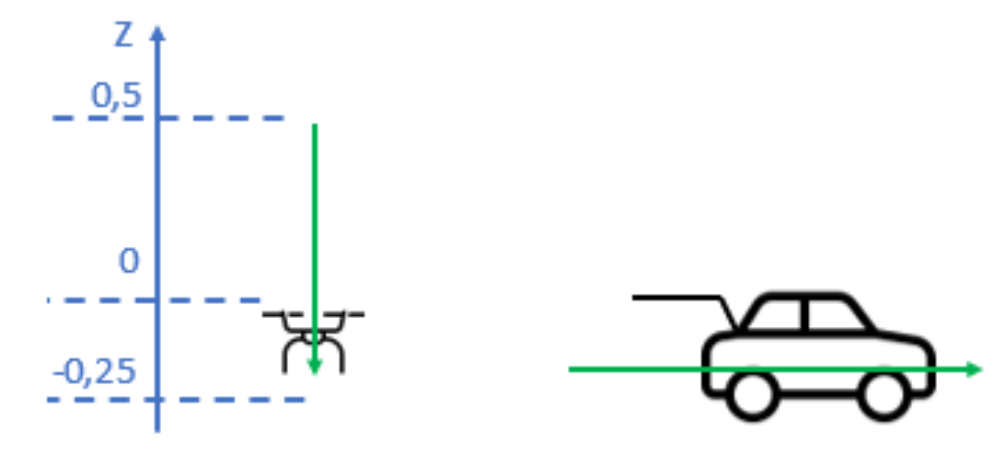
\includegraphics[
                width=\linewidth,
                height=1.65cm,
                keepaspectratio
            ]{step_3.png}
        \end{column}

        \begin{column}{0.62\textwidth}
            \centering
            \includegraphics[
                width=0.96\linewidth,
                height=0.64\textheight,
                keepaspectratio
            ]{asservissement position ekf présence de bruit.png}
        \end{column}
    \end{columns}
\end{frame}

% ==============================================================================
% CONTROLLER COMPARISON
% ==============================================================================

\begin{frame}{Comparison}
    \framesubtitle{LQ, MPC and MPC with EKF}

    \begin{columns}[T,onlytextwidth]
        \begin{column}{0.31\textwidth}
            \begin{block}{LQ control}
                \begin{itemize}
                    \item Simple and computationally efficient.
                    \item Based on a linear model.
                    \item No state measurement feedback.
                \end{itemize}
            \end{block}
        \end{column}

        \begin{column}{0.31\textwidth}
            \begin{block}{MPC control}
                \begin{itemize}
                    \item Uses a predictive RNN model.
                    \item Handles nonlinear dynamics.
                    \item No EKF state correction.
                \end{itemize}
            \end{block}
        \end{column}

        \begin{column}{0.31\textwidth}
            \begin{exampleblock}{MPC with EKF}
                \begin{itemize}
                    \item Corrected state estimation.
                    \item Feedback from measurements.
                    \item Improved robustness.
                \end{itemize}
            \end{exampleblock}
        \end{column}
    \end{columns}
\end{frame}

% ==============================================================================
% SECTION 11: PRBS DATA GENERATION
% ==============================================================================
\section{Advanced Control Law}

\begin{frame}{Data generation}
    \framesubtitle{PRBS excitation in the 3D drone workspace}

    \begin{columns}[T,onlytextwidth]

        \begin{column}{0.48\textwidth}
            \begin{block}{Objective}
                Generate sufficiently rich input/output trajectories to
                identify a nonlinear dynamic model of the drone.
                \begin{itemize}
                    \item Excite the four actuator commands around hover
                    \item Capture the coupled 3D dynamics (12 variables)
                    \item Store synchronized inputs and measured outputs
                \end{itemize}
            \end{block}

            \begin{block}{Simulation setup}
                \begin{itemize}
                    \item Sampling time: $T_s = 0.05\,\mathrm{s}$
                    \item $N = 2000$ samples per trajectory
                    \item $3000$ independent experiments
                    \item Initial hover command: $U_{\mathrm{hover}} = 0.55$
                \end{itemize}
            \end{block}
        \end{column}

        \begin{column}{0.48\textwidth}
            \begin{block}{APRBS modes}
                We don't directly generate u inputs (unusable data).
                Instead, we use a flight controller : the inputs are now four independently generated piecewise-constant modes:
                \[
                    \delta = [\delta_T,\delta_r,\delta_p,\delta_y]
                \]

                Each level is sampled uniformly and held for a random duration
                between $1$ and $3$ seconds.
            \end{block}
        \end{column}
    \end{columns}
\end{frame}

\begin{frame}{Data generation}
    \framesubtitle{Flight controller}
    \begin{columns}[T,onlytextwidth]
        \begin{column}{0.50\textwidth}
            \begin{block}{From version 1 to version 2}
                The first version used PID controllers directly on the
                attitude angles. This solution was stable, but not fast
                enough for the drone dynamics (see appendix).

                Version 2 therefore uses a cascade controller: an outer
                angle loop generates an angular-rate reference, followed by
                a fast inner PID loop based on the gyroscope measurement.
            \end{block}

            \begin{block}{Controller parameters}
                \begin{itemize}
                    \item Outer angle gain: $K_a=2.5$
                    \item Inner rate PID:
                    $P=0.125,\ I=0.05,\ D=0.025,\ N=100$
                    \item Sampling time: $T_s=0.005\,\mathrm{s}$
                    \item Same structure for roll and pitch
                \end{itemize}
            \end{block}
        \end{column}

        \begin{column}{0.49\textwidth}
            \centering
            \resizebox{\linewidth}{!}{%
            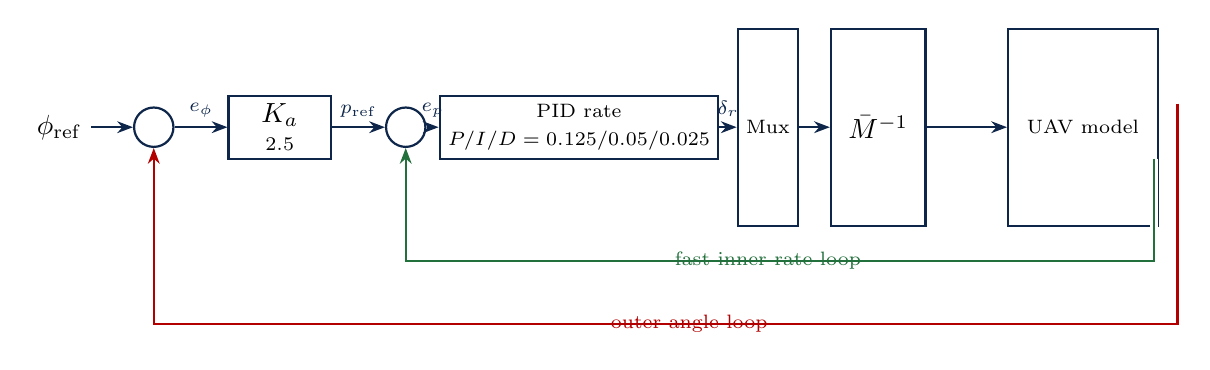
\begin{tikzpicture}[
                blk/.style={draw=CSNavy,thick,fill=white,align=center,
                    inner sep=3pt,minimum height=8mm},
                sum/.style={circle,draw=CSNavy,thick,fill=white,
                    minimum size=5mm,inner sep=0pt},
                sig/.style={->,thick,CSNavy},
                rate/.style={->,thick,DarkGreen},
                angle/.style={->,thick,red!70!black},
                >={Stealth[length=2mm]},
                hop/.style={preaction={draw=white,line width=3pt}}]
                \node (ref) at (0,0) {$\phi_{\mathrm{ref}}$};
                \node[sum] (s1) at (1.2,0) {};
                \node[blk,minimum width=13mm] (ka) at (2.8,0)
                    {$K_a$\\[-2pt]\scriptsize $2.5$};
                \node[sum] (s2) at (4.4,0) {};
                \node[blk,minimum width=22mm] (pid) at (6.6,0)
                    {\scriptsize PID rate\\[-2pt]
                    \scriptsize $P/I/D=0.125/0.05/0.025$};
                \node[blk,minimum width=5mm,minimum height=25mm] (mux)
                    at (9.0,0) {\scriptsize Mux};
                \node[blk,minimum width=12mm,minimum height=25mm] (mix)
                    at (10.4,0) {$\bar M^{-1}$};
                \node[blk,minimum width=19mm,minimum height=25mm] (uav)
                    at (13.0,0) {\scriptsize UAV model};

                \draw[sig] (ref) -- (s1);
                \draw[sig] (s1) -- node[above,font=\scriptsize]{$e_\phi$} (ka);
                \draw[sig] (ka) -- node[above,font=\scriptsize]{$p_{\rm ref}$} (s2);
                \draw[sig] (s2) -- node[above,font=\scriptsize]{$e_p$} (pid);
                \draw[sig] (pid) -- node[above,font=\scriptsize]{$\delta_r$}
                    (mux);
                \draw[sig] (mux) -- (mix);
                \draw[sig] (mix) -- (uav);

                \draw[rate,hop] (13.9,-0.4) -- (13.9,-1.7) -- (4.4,-1.7)
                    -- (s2.south);
                \draw[angle,hop] (14.2,0.3) -- (14.2,-2.5) -- (1.2,-2.5)
                    -- (s1.south);
                \node[font=\scriptsize,DarkGreen] at (9,-1.7)
                    {fast inner rate loop};
                \node[font=\scriptsize,red!70!black] at (8,-2.5)
                    {outer angle loop};
            \end{tikzpicture}}
        \end{column}
    \end{columns}
\end{frame}

% ==============================================================================
% ADVANCED CONTROL LAW: NEW RNN, 3D MPC AND 3D EKF
% ==============================================================================

% ------------------------------------------------------------------------------
% NEW RNN MODEL
% ------------------------------------------------------------------------------
\begin{frame}{New RNN model}
    \framesubtitle{Trained on flight controller + drone simulations}

    \begin{columns}[T,onlytextwidth]
        \begin{column}{0.5\textwidth}
            \begin{block}{What the RNN learns}
                \centering
                \resizebox{\linewidth}{!}{%
                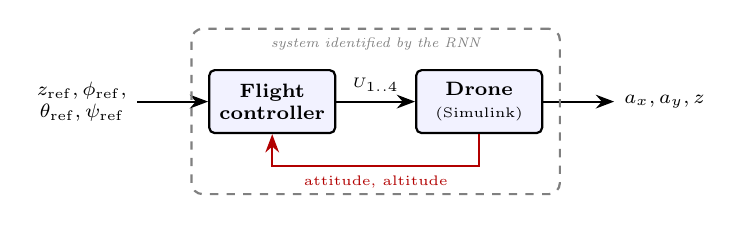
\begin{tikzpicture}[
                    >=Stealth, thick,
                    block/.style={draw, rectangle, minimum height=0.8cm,
                        minimum width=1.6cm, align=center, fill=blue!5,
                        rounded corners=2pt, font=\scriptsize}
                ]
                    \node[block] (fc) {\textbf{Flight}\\\textbf{controller}};
                    \node[block, right=1.0cm of fc] (drone) {\textbf{Drone}\\\tiny (Simulink)};
                    \draw[->] (fc) -- node[above, font=\tiny] {$U_{1..4}$} (drone);
                    \draw[->] ([xshift=-0.9cm]fc.west)
                        node[left, font=\scriptsize, align=center]
                        {$z_{\mathrm{ref}}, \phi_{\mathrm{ref}},$\\
                         $\theta_{\mathrm{ref}}, \psi_{\mathrm{ref}}$}
                        -- (fc.west);
                    \draw[->] (drone.east) -- ++(0.9,0)
                        node[right, font=\scriptsize] {$a_x, a_y, z$};
                    \draw[->, red!70!black] (drone.south) -- ++(0,-0.4) -|
                        node[pos=0.25, below, font=\tiny] {attitude, altitude} (fc.south);
                    \node[draw, dashed, gray, rounded corners, inner sep=6pt,
                        fit={(fc) (drone) ([yshift=-0.55cm]drone.south)
                             ([yshift=0.3cm]fc.north)}] (box) {};
                    \node[gray, font=\tiny\itshape, anchor=north]
                        at (box.north) {system identified by the RNN};
                \end{tikzpicture}%
                }
            \end{block}

            \begin{block}{Model and training}
                \footnotesize
                \begin{itemize}\setlength{\itemsep}{0pt}
                    \item Elman RNN, 32 hidden units, 1.3\,k parameters
                    \item 4 inputs $\rightarrow$ 3 outputs $(a_x, a_y, z)$
                    \item 3000 trajectories of 1941 steps, 70\,\% for training
                    \item Adam, $\mathrm{lr}=10^{-3}$, 100 epochs, batch 32
                    \item Test RMSE: $a_x$ 0.24, $a_y$ 0.23\,m/s$^2$,
                    $z$ 0.048\,m
                \end{itemize}
            \end{block}
        \end{column}

        \begin{column}{0.47\textwidth}
            \begin{alertblock}{Why a new model?}
                \footnotesize
                \begin{itemize}\setlength{\itemsep}{0pt}
                    \item The first RNN only described the $z$ axis
                    ($u \rightarrow a_z$).
                    \item 3D control needs $x$ and $y$, but raw motor data is
                    unusable (unstable drone).
                    \item With the flight controller inside, the identified
                    system is stable, with bounded physical inputs.
                    \item The MPC sends references to the flight
                    controller, like an autopilot.
                \end{itemize}
            \end{alertblock}

            \begin{block}{Choice of the outputs}
                \footnotesize
                \begin{itemize}\setlength{\itemsep}{0pt}
                    \item $z$ is held by the altitude loop: learned
                    directly, no double integration (lesson from $a_z$).
                    \item No position loop on $x, y$: learn $a_x, a_y$, then
                    integrate.
                \end{itemize}
            \end{block}
        \end{column}
    \end{columns}
\end{frame}

% ------------------------------------------------------------------------------
% 3D MPC
% ------------------------------------------------------------------------------
\begin{frame}{3D MPC}
    \framesubtitle{Position control through the flight controller}

    \begin{columns}[T,onlytextwidth]
        \begin{column}{0.52\textwidth}
            \begin{block}{Cost function minimized}
                \footnotesize
                \setlength{\abovedisplayskip}{0pt}\setlength{\belowdisplayskip}{2pt}
                \[
                    J(U) = \sum_{i=1}^{N} Q\,\big\|\hat{p}_{k+i} - r_{k+i}\big\|^2
                    + R\,\big\|u_{k+i-1} - u_{k+i-2}\big\|^2
                \]
                {\scriptsize\raggedright
                $\hat{p}=(\hat{x}, \hat{y}, \hat{z})$: position predicted
                with the RNN\\
                $u = (z_{\mathrm{ref}}, \phi_{\mathrm{ref}},
                \theta_{\mathrm{ref}}, \psi_{\mathrm{ref}})$: references
                sent to the flight controller\\
                $r$: 3D reference trajectory\par}
            \end{block}

            \begin{block}{Prediction over the horizon}
                \footnotesize
                \setlength{\abovedisplayskip}{0pt}\setlength{\belowdisplayskip}{2pt}
                \begin{align*}
                    (a_{x}, a_{y}, z)_{k} &= \mathrm{RNN}(h_{k-1}, u_{k-1})\\
                    v_{k} &= v_{k-1} + a_{k}\,\Delta t \quad (x, y)\\
                    p_{k} &= p_{k-1} + v_{k}\,\Delta t \quad (x, y)
                \end{align*}
                {\scriptsize $z$ is read directly from the RNN output.\par}
            \end{block}
        \end{column}

        \begin{column}{0.45\textwidth}
            \begin{block}{Constraints}
                \footnotesize
                $u_{\min} \le u \le u_{\max}$: the range seen in training
                \begin{itemize}\setlength{\itemsep}{0pt}
                    \item $z_{\mathrm{ref}} \in [0.5,\ 2.5]$\,m
                    \item $\phi_{\mathrm{ref}}, \theta_{\mathrm{ref}}
                    \in [-0.3,\ 0.3]$\,rad
                    \item $\psi_{\mathrm{ref}} \in [-0.5,\ 0.5]$\,rad
                \end{itemize}
                {\scriptsize Outside this range the RNN would extrapolate.\par}
            \end{block}

            \begin{exampleblock}{Settings}
                \footnotesize
                \begin{itemize}\setlength{\itemsep}{0pt}
                    \item 50 Adam steps per sample ($\mathrm{lr}=0.05$),
                    warm start
                    \item $T_e = 0.05$\,s, $Q = R = 1$
                    \item $N=20$ (1\,s): with $N=10$ (0.5\,s) the MPC diverges
                \end{itemize}
            \end{exampleblock}
        \end{column}
    \end{columns}
\end{frame}


% ------------------------------------------------------------------------------
% Closing Slide (same background as the title slide)
% ------------------------------------------------------------------------------
{
\setbeamertemplate{background}{%
    \begin{tikzpicture}[remember picture, overlay]
        \clip (current page.south west) rectangle (current page.north east);
        \node[at=(current page.center), opacity=0.20, inner sep=0pt] {
            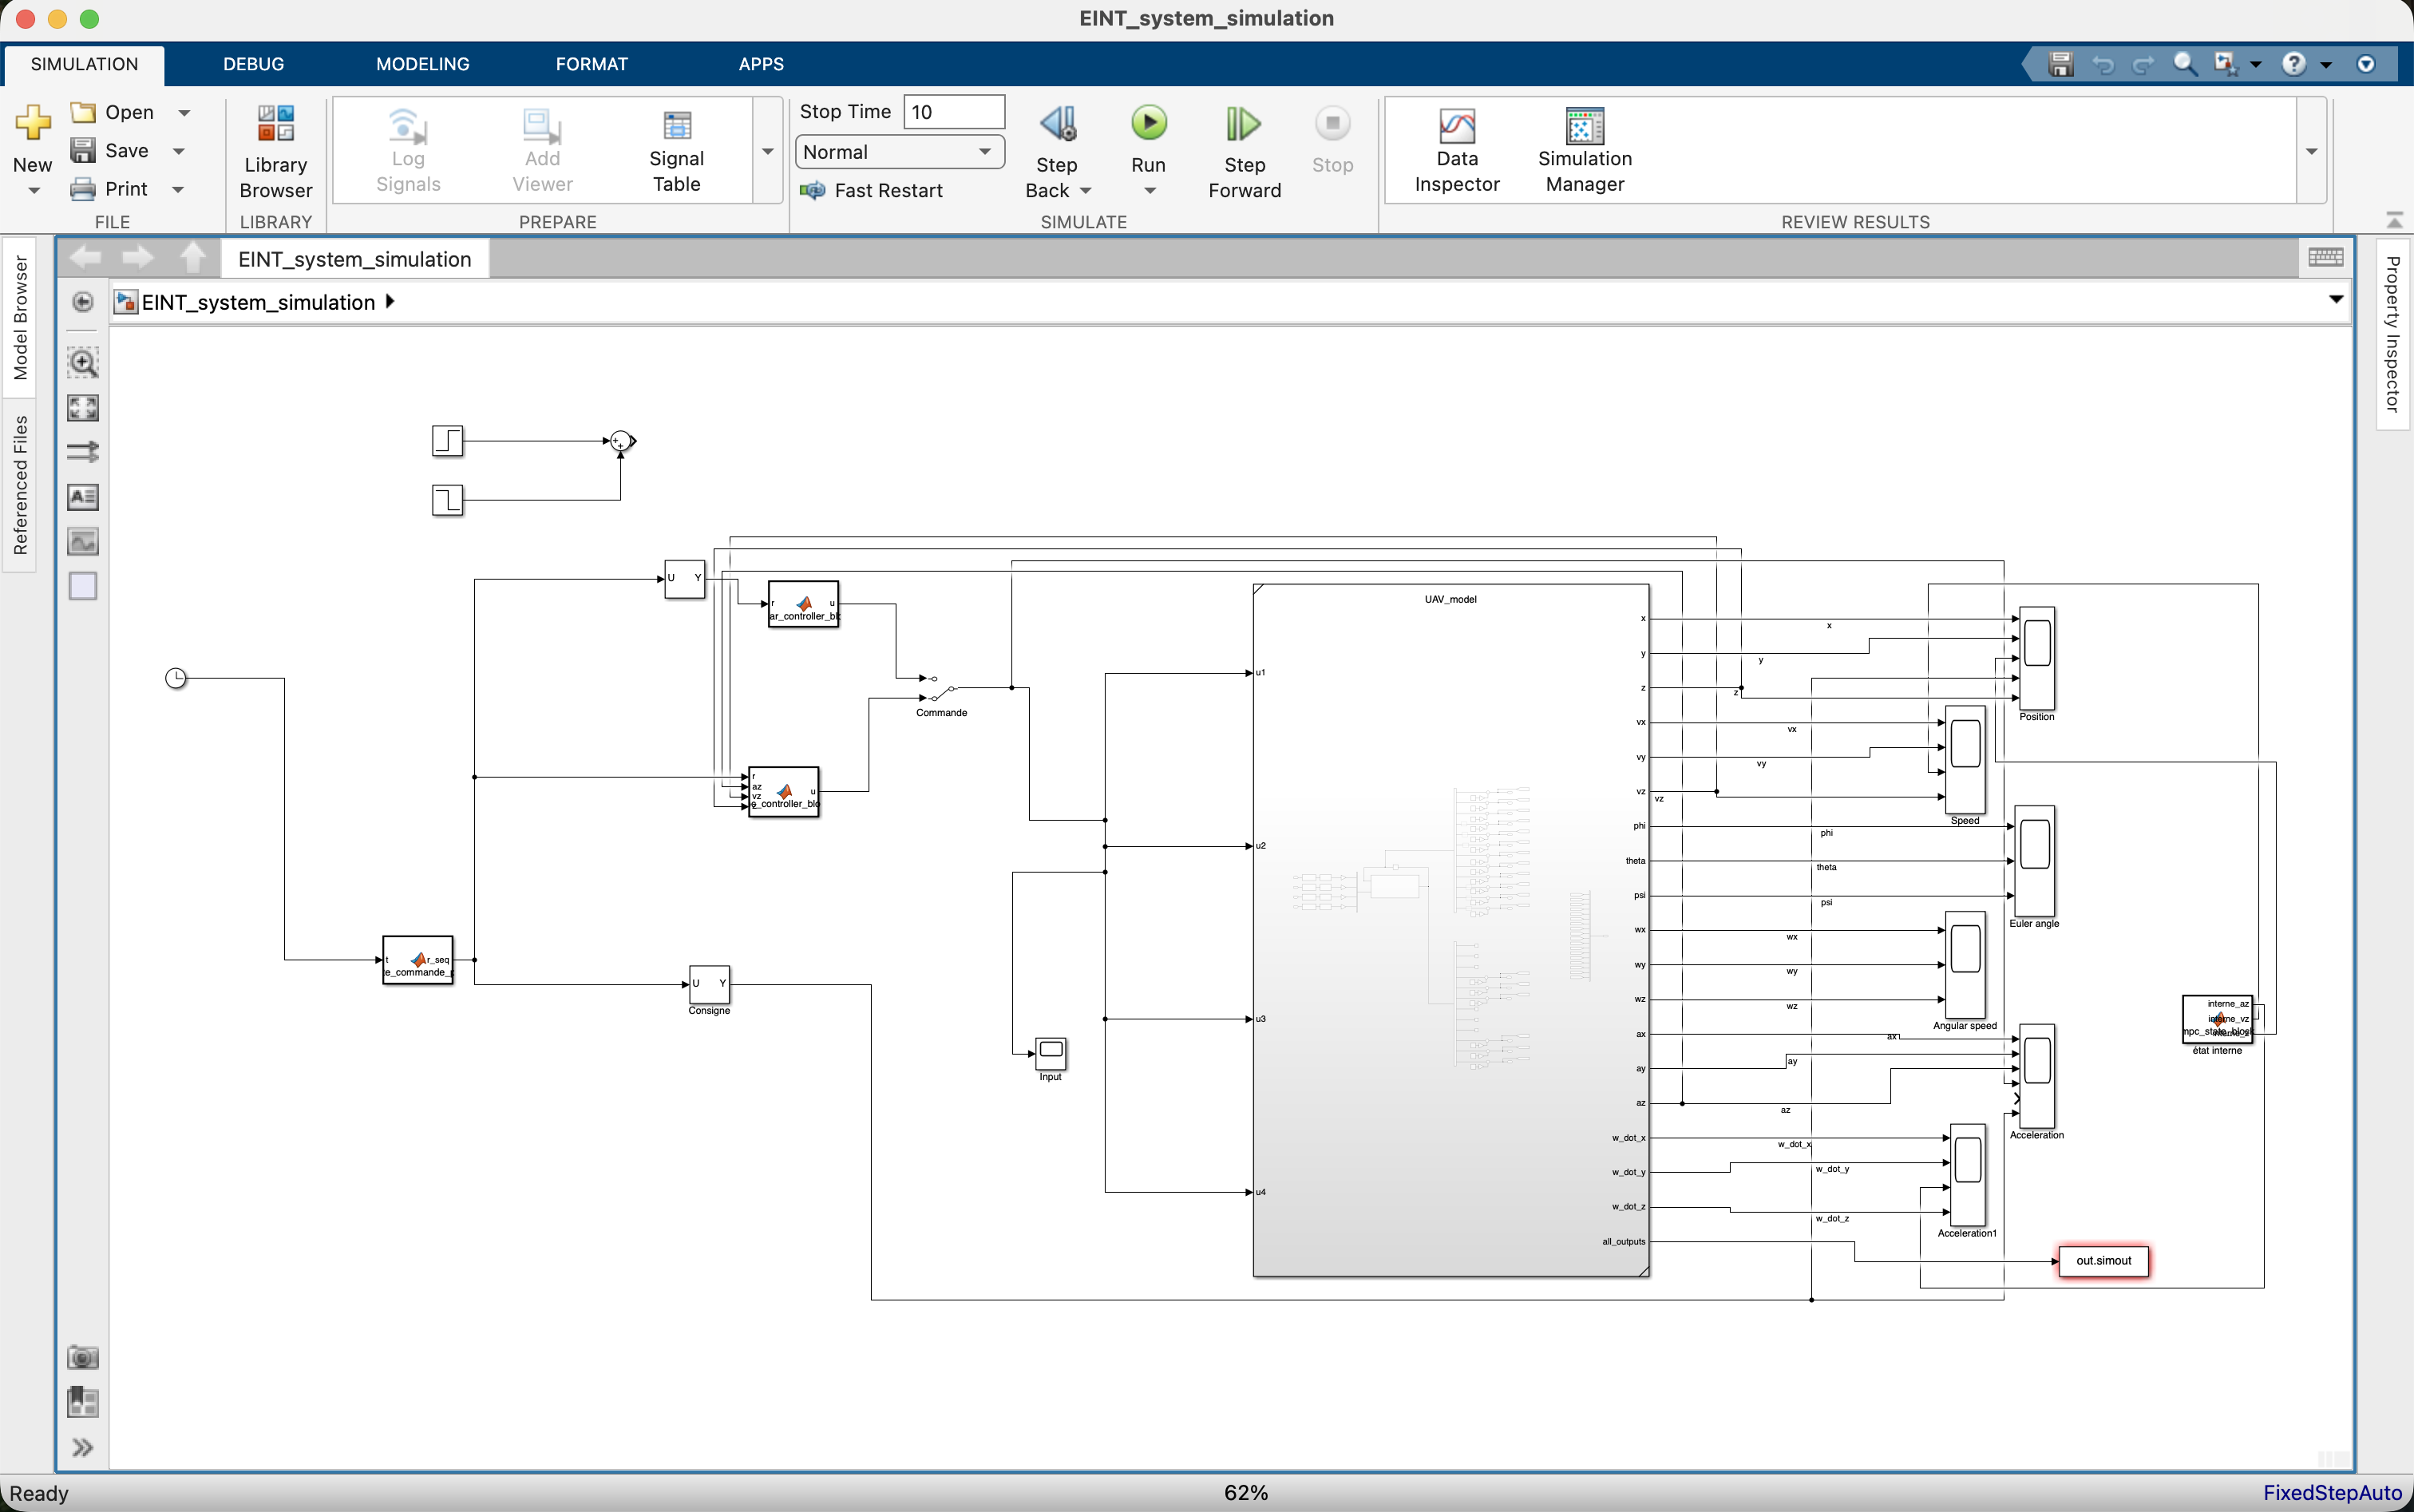
\includegraphics[width=\paperwidth]{screen_simulink.png}
        };
    \end{tikzpicture}%
}
\begin{frame}[plain,noframenumbering]
    \centering
    \vfill
    {\usebeamerfont{title}\color{CSNavy}\LARGE\bfseries Thank you for your attention}

    \vspace{0.8cm}
    {\Large\color{CSSlate} Questions?}

    \vspace{1.2cm}
    {\small \insertauthor}

    \vspace{0.3cm}
    {\footnotesize\color{gray} \insertinstitute{} -- \insertdate}
    \vfill
\end{frame}
}

% ==============================================================================
% APPENDIX
% ==============================================================================
\appendix
\section{Appendix}

\begin{frame}{Appendix: System Modeling}
    \framesubtitle{Linear Model: Least Square Method}
    \begin{columns}[T]
        \begin{column}{0.52\textwidth}

            \begin{block}{Model equations}
                \begin{align*}
                    y_k(t+1)
                        &= a\,y_k(t) + b\,u_k(t) + c \\
                        &= \boldsymbol{\varphi}_k^{\mathsf T}
                           \boldsymbol{\theta}.
                \end{align*}
                \[
                    \boldsymbol{\varphi}_k^{\mathsf T} =
                    \begin{bmatrix} y_k(t) & u_k(t) & 1 \end{bmatrix}
                    \qquad
                    \boldsymbol{\theta} =
                    \begin{bmatrix} a & b & c \end{bmatrix}^{\mathsf T}.
                \]

                The least-squares estimate is
                \begin{equation*}
                    \boldsymbol{\theta}^{\star}
                        =
                        \left(\boldsymbol{\Phi}^{\mathsf T}
                        \boldsymbol{\Phi}\right)^{-1}
                        \boldsymbol{\Phi}^{\mathsf T}\boldsymbol{Y}.
                \end{equation*}
            \end{block}
        \end{column}

        \begin{column}{0.48\textwidth}
            \centering

            \vspace{0.15cm}

            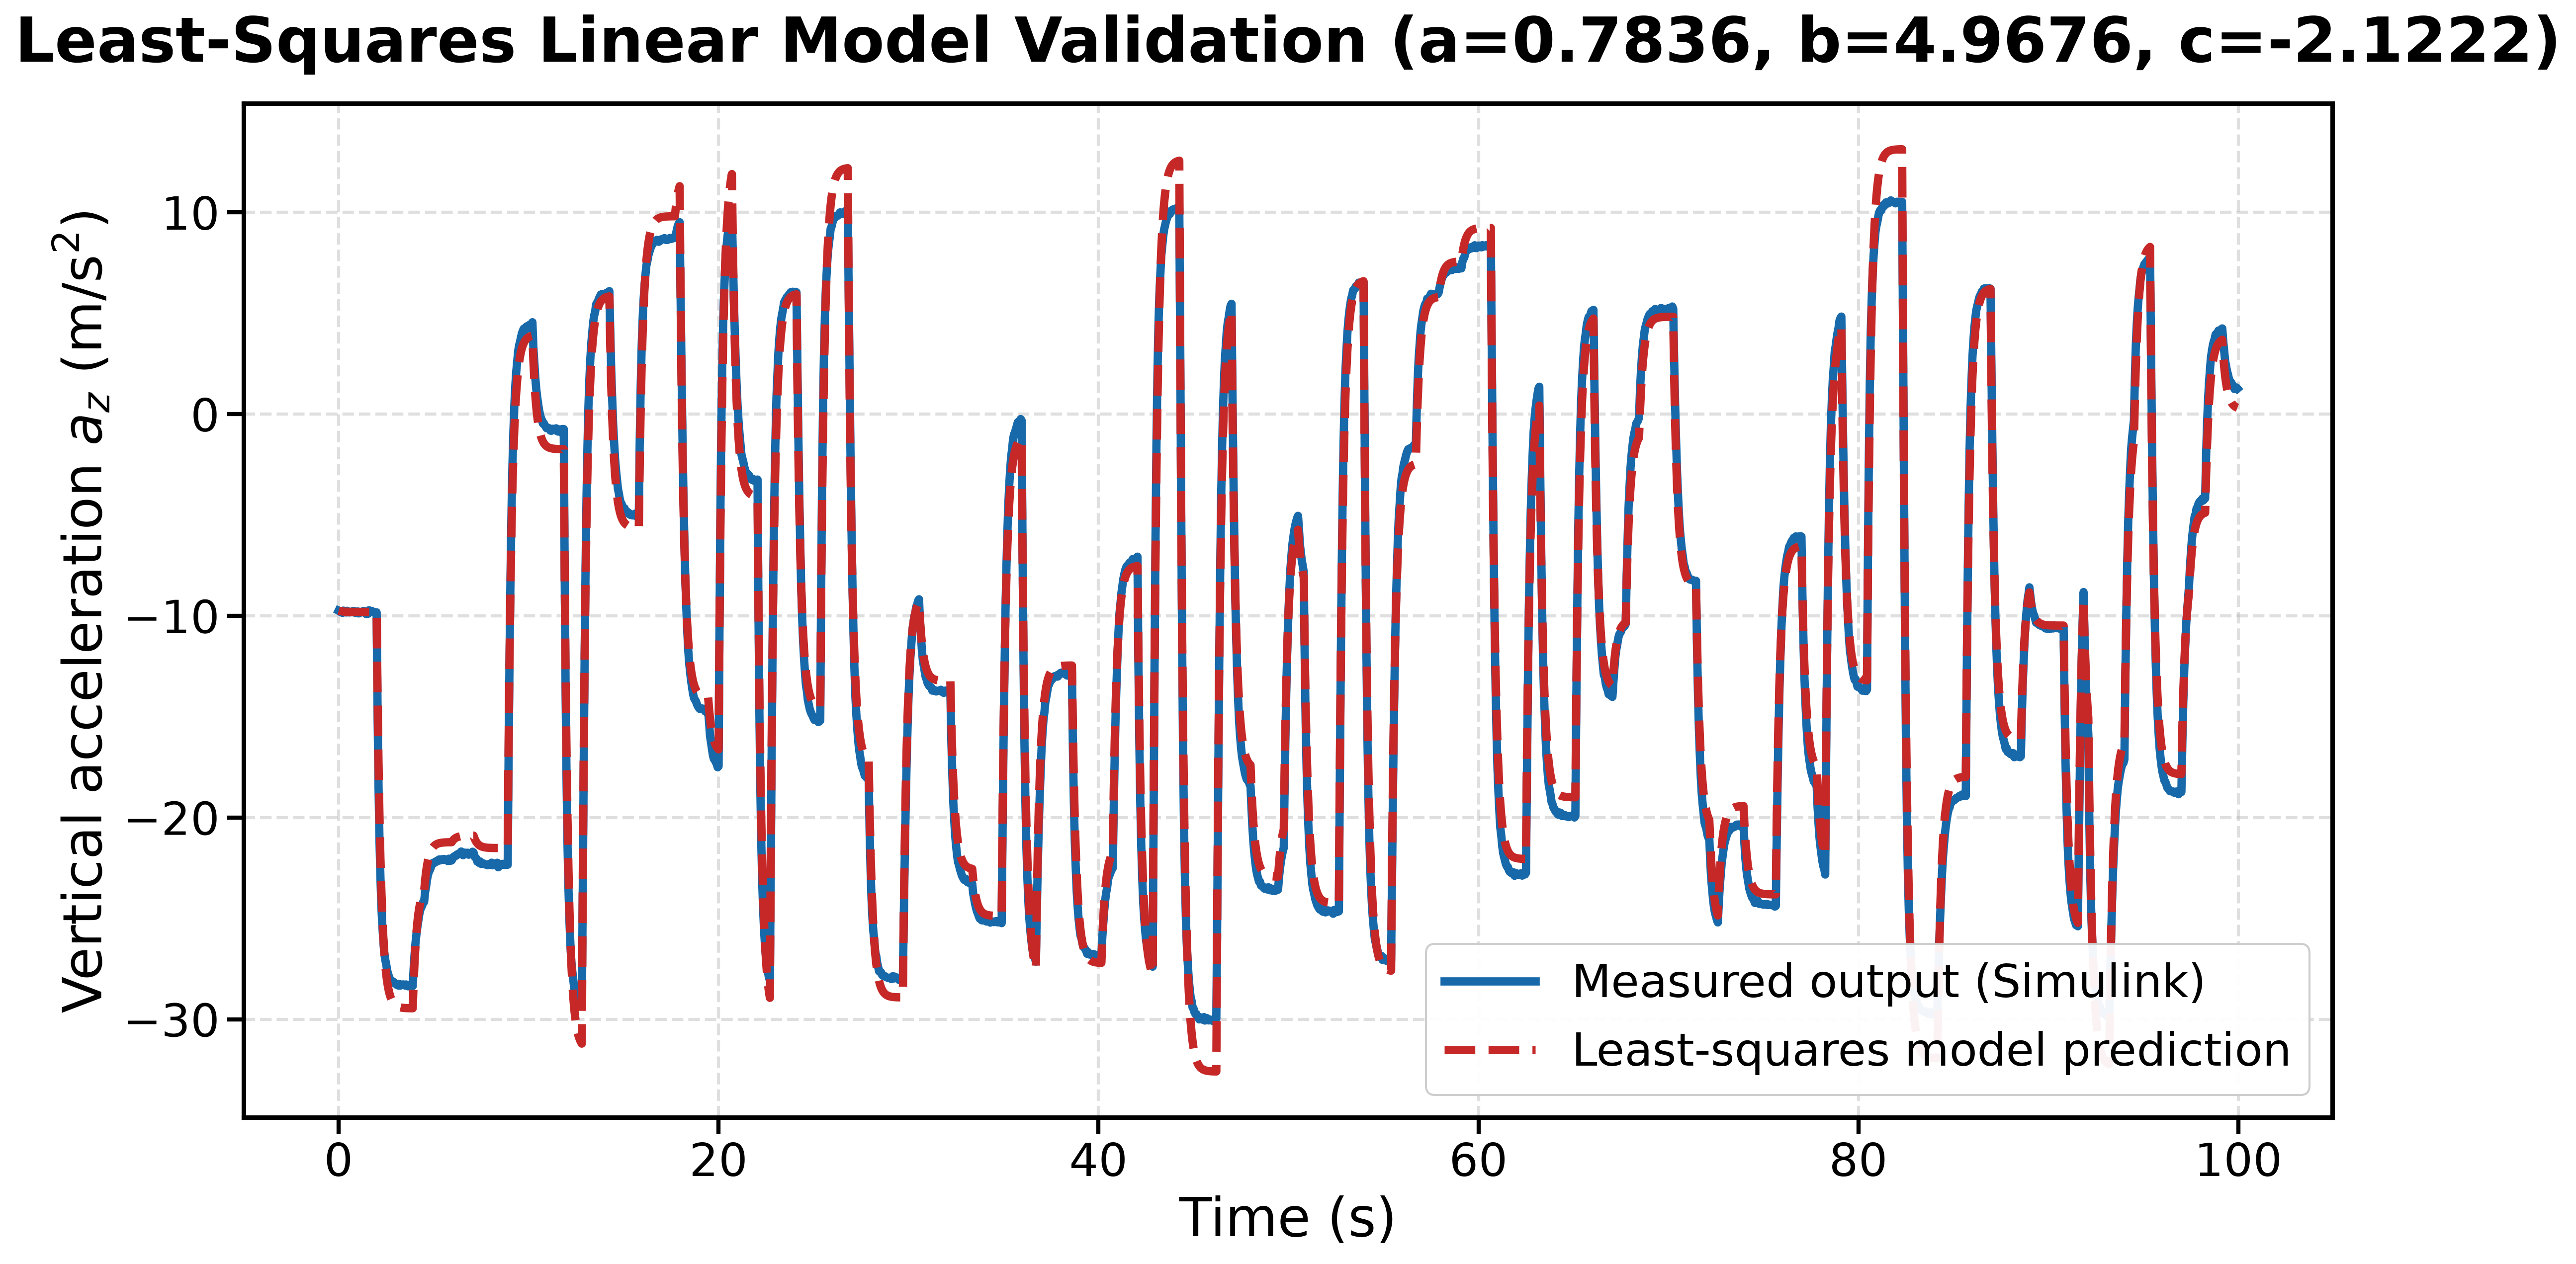
\includegraphics[
                width=\linewidth,
                height=2.75cm,
                keepaspectratio
            ]{least_squares_validation.png}
        \end{column}
    \end{columns}
\end{frame}

\begin{frame}{Appendix: System Modeling}
    \framesubtitle{Linear Model with Constant Steady-State Gain}
    \begin{columns}[T]
        \begin{column}{0.54\textwidth}
            \small
            \begin{block}{State Function}
                First-order lag driven by a constant gain $K$ and offset $c$:
                $\dot{v}(t) = \frac{1}{\tau}\bigl(K u(t) - v(t)\bigr)$,
                i.e.\ $\tau\,\dot{v} + v = K u + c$.
            \end{block}
            \begin{block}{Parameter Identification}
                - \textbf{Static gain $K$}: affine least-squares fit on steady-state regimes:
                \begin{equation*}
                    v(t) = K\,u(t) + c, \qquad K \approx 22.5,\ c \approx -9.8
                \end{equation*}
                - \textbf{Tau identification}
            \end{block}
        \end{column}

        \begin{column}{0.46\textwidth}

                \centering
                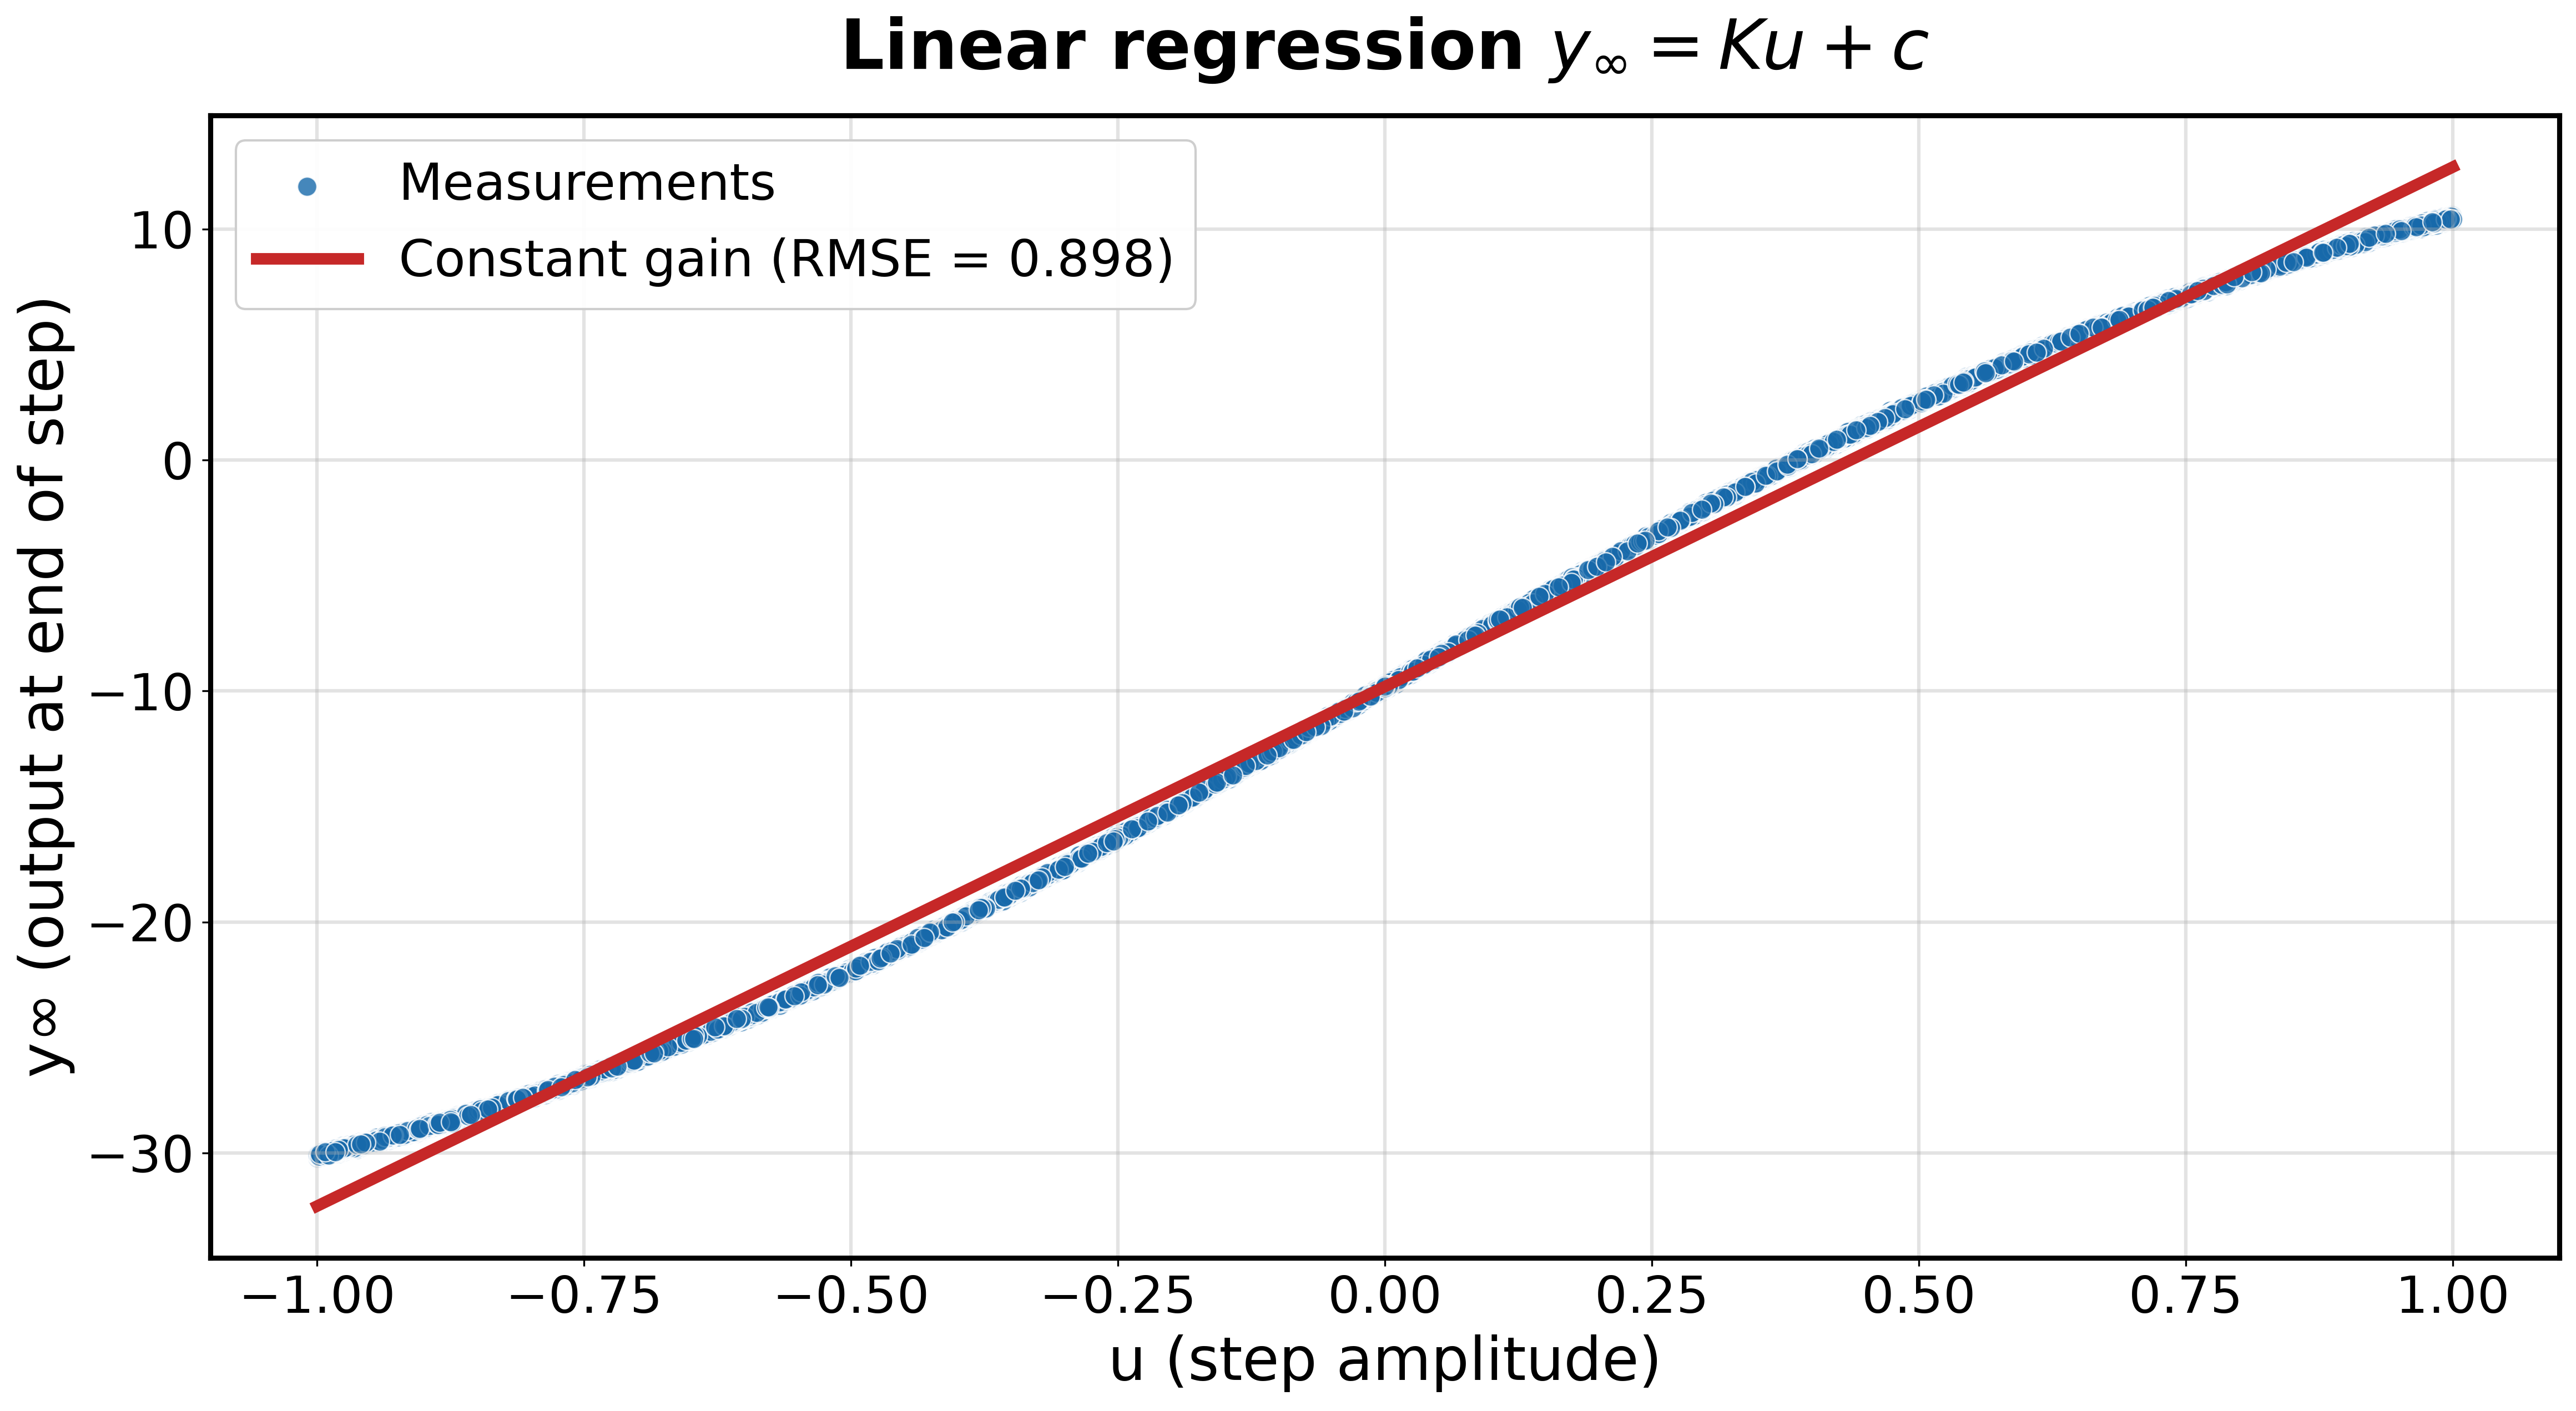
\includegraphics[
                    width=\linewidth,
                    height=2.3cm,
                    keepaspectratio
                ]{constant_gain_regression.png}


                \centering
                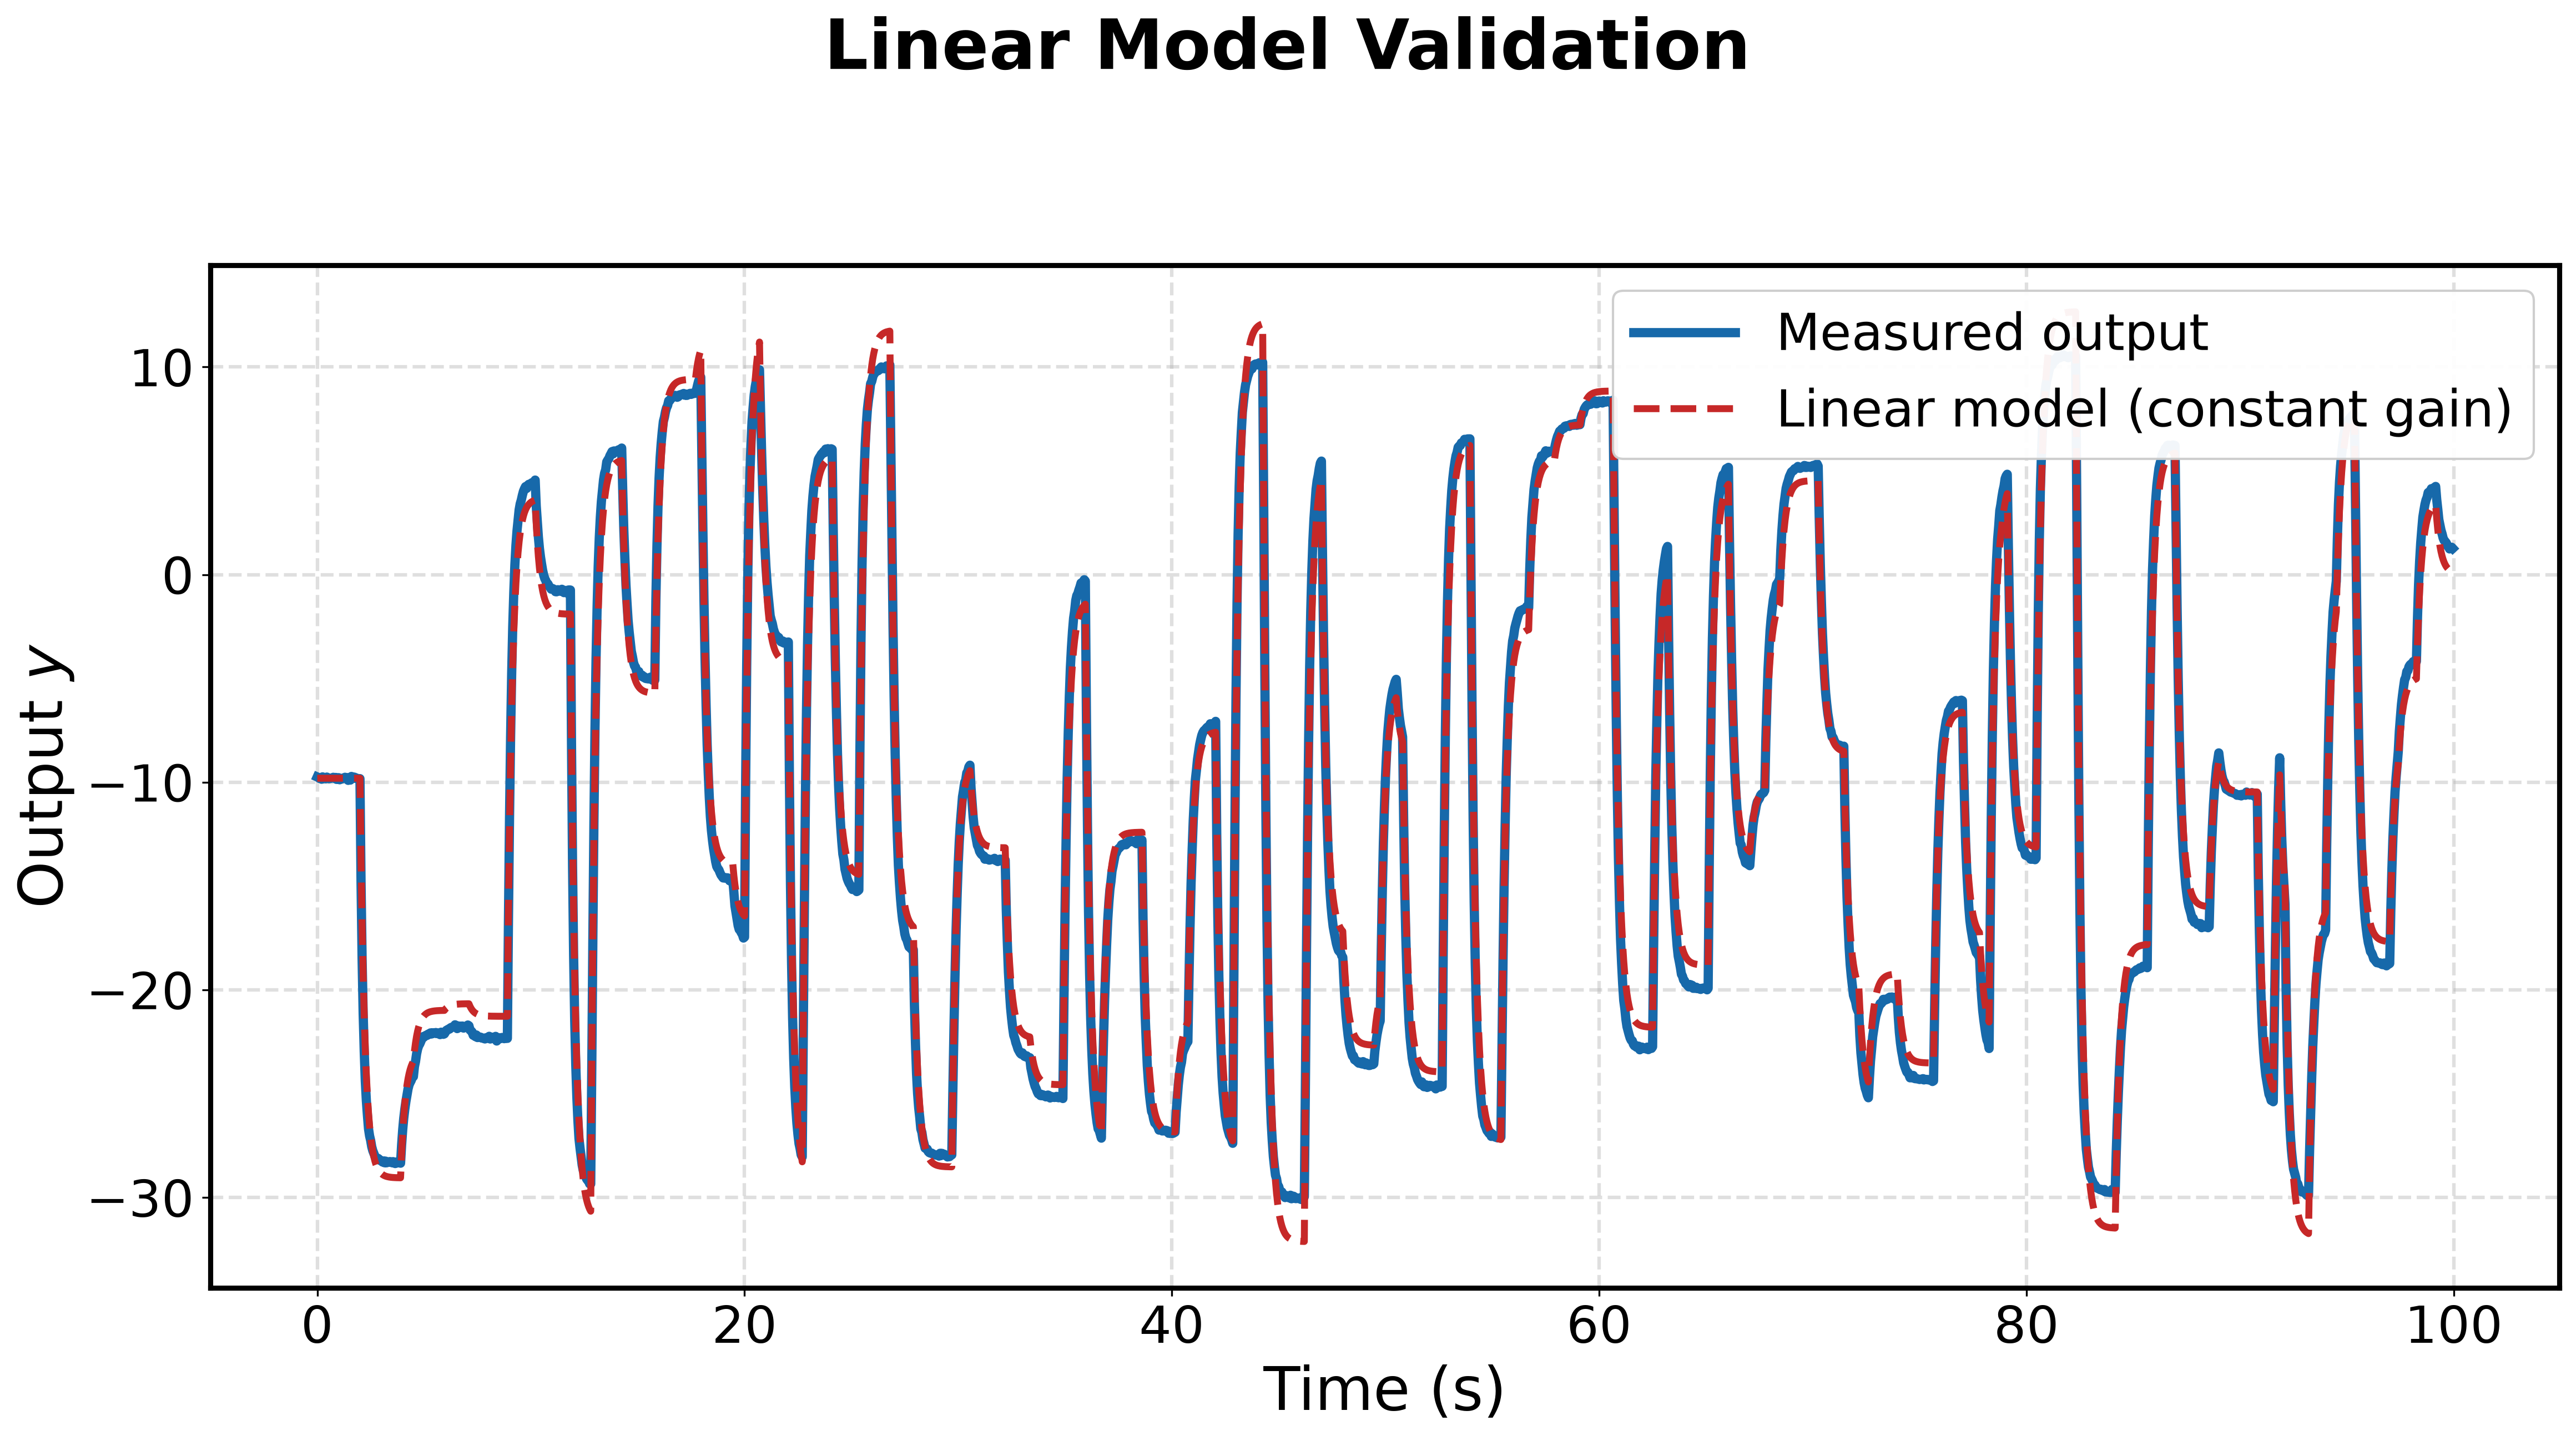
\includegraphics[
                    width=\linewidth,
                    height=6.2cm,
                    keepaspectratio
                ]{linear_gain_validation.png}
        \end{column}
    \end{columns}
\end{frame}

\begin{frame}{Appendix: Extended Kalman Filter}
    \framesubtitle{Predict and update steps}
    \begin{columns}[T,onlytextwidth]
        \begin{column}{0.48\textwidth}
            \begin{block}{Predict}
                \footnotesize
                \vspace{-6pt}
                \begin{align*}
                    \hat{x}_{k|k-1} &= f(\hat{x}_{k-1|k-1},u_{k-1})\\
                    P_{k|k-1} &= F_k P_{k-1|k-1} F_k^\top + Q,\quad F_k=\tfrac{\partial f}{\partial x}
                \end{align*}
            \end{block}
        \end{column}
        \begin{column}{0.48\textwidth}
            \begin{block}{Update}
                \footnotesize
                \vspace{-6pt}
                \begin{align*}
                    K_k &= P_{k|k-1} H^\top (H P_{k|k-1} H^\top + R)^{-1}\\
                    \hat{x}_{k|k} &= \hat{x}_{k|k-1} + K_k\,(y_k - H\hat{x}_{k|k-1} - c)\\
                    P_{k|k} &= (I-K_kH)\,P_{k|k-1}
                \end{align*}
            \end{block}
        \end{column}
    \end{columns}
\end{frame}


\end{document}
